\documentclass[twoside]{book}

% Packages required by doxygen
\usepackage{fixltx2e}
\usepackage{calc}
\usepackage{doxygen}
\usepackage[export]{adjustbox} % also loads graphicx
\usepackage{graphicx}
\usepackage[utf8]{inputenc}
\usepackage{makeidx}
\usepackage{multicol}
\usepackage{multirow}
\PassOptionsToPackage{warn}{textcomp}
\usepackage{textcomp}
\usepackage[nointegrals]{wasysym}
\usepackage[table]{xcolor}

% Font selection
\usepackage[T1]{fontenc}
\usepackage[scaled=.90]{helvet}
\usepackage{courier}
\usepackage{amssymb}
\usepackage{sectsty}
\renewcommand{\familydefault}{\sfdefault}
\allsectionsfont{%
  \fontseries{bc}\selectfont%
  \color{darkgray}%
}
\renewcommand{\DoxyLabelFont}{%
  \fontseries{bc}\selectfont%
  \color{darkgray}%
}
\newcommand{\+}{\discretionary{\mbox{\scriptsize$\hookleftarrow$}}{}{}}

% Page & text layout
\usepackage{geometry}
\geometry{%
  a4paper,%
  top=2.5cm,%
  bottom=2.5cm,%
  left=2.5cm,%
  right=2.5cm%
}
\tolerance=750
\hfuzz=15pt
\hbadness=750
\setlength{\emergencystretch}{15pt}
\setlength{\parindent}{0cm}
\setlength{\parskip}{3ex plus 2ex minus 2ex}
\makeatletter
\renewcommand{\paragraph}{%
  \@startsection{paragraph}{4}{0ex}{-1.0ex}{1.0ex}{%
    \normalfont\normalsize\bfseries\SS@parafont%
  }%
}
\renewcommand{\subparagraph}{%
  \@startsection{subparagraph}{5}{0ex}{-1.0ex}{1.0ex}{%
    \normalfont\normalsize\bfseries\SS@subparafont%
  }%
}
\makeatother

% Headers & footers
\usepackage{fancyhdr}
\pagestyle{fancyplain}
\fancyhead[LE]{\fancyplain{}{\bfseries\thepage}}
\fancyhead[CE]{\fancyplain{}{}}
\fancyhead[RE]{\fancyplain{}{\bfseries\leftmark}}
\fancyhead[LO]{\fancyplain{}{\bfseries\rightmark}}
\fancyhead[CO]{\fancyplain{}{}}
\fancyhead[RO]{\fancyplain{}{\bfseries\thepage}}
\fancyfoot[LE]{\fancyplain{}{}}
\fancyfoot[CE]{\fancyplain{}{}}
\fancyfoot[RE]{\fancyplain{}{\bfseries\scriptsize Generated by Doxygen }}
\fancyfoot[LO]{\fancyplain{}{\bfseries\scriptsize Generated by Doxygen }}
\fancyfoot[CO]{\fancyplain{}{}}
\fancyfoot[RO]{\fancyplain{}{}}
\renewcommand{\footrulewidth}{0.4pt}
\renewcommand{\chaptermark}[1]{%
  \markboth{#1}{}%
}
\renewcommand{\sectionmark}[1]{%
  \markright{\thesection\ #1}%
}

% Indices & bibliography
\usepackage{natbib}
\usepackage[titles]{tocloft}
\setcounter{tocdepth}{3}
\setcounter{secnumdepth}{5}
\makeindex

% Hyperlinks (required, but should be loaded last)
\usepackage{ifpdf}
\ifpdf
  \usepackage[pdftex,pagebackref=true]{hyperref}
\else
  \usepackage[ps2pdf,pagebackref=true]{hyperref}
\fi
\hypersetup{%
  colorlinks=true,%
  linkcolor=blue,%
  citecolor=blue,%
  unicode%
}

% Custom commands
\newcommand{\clearemptydoublepage}{%
  \newpage{\pagestyle{empty}\cleardoublepage}%
}

\usepackage{caption}
\captionsetup{labelsep=space,justification=centering,font={bf},singlelinecheck=off,skip=4pt,position=top}

%===== C O N T E N T S =====

\begin{document}

% Titlepage & ToC
\hypersetup{pageanchor=false,
             bookmarksnumbered=true,
             pdfencoding=unicode
            }
\pagenumbering{roman}
\begin{titlepage}
\vspace*{7cm}
\begin{center}%
{\Large A\+PI K\+A\+C\+HU }\\
\vspace*{1cm}
{\large Generated by Doxygen 1.8.11}\\
\end{center}
\end{titlepage}
\clearemptydoublepage
\tableofcontents
\clearemptydoublepage
\pagenumbering{arabic}
\hypersetup{pageanchor=true}

%--- Begin generated contents ---
\chapter{A\+P\+I\+Kachu}
\label{index}\hypertarget{index}{}Welcome to \hyperlink{namespace_a_p_i_kachu}{A\+P\+I\+Kachu}\textquotesingle{}s documentation. You can find a list of classes and their methods in the toolbar above.

To create a module, you have to implement the I\+Module interface and its methods accordingly. You\textquotesingle{}ll find more details in the documentation of the class.

First of all, when the server receives a new connection, it should create an instance of I\+Http\+Client containing the IP address of the client as an I\+I\+P\+Address. This is to be used later on by the modules if needed. Note that all enabled modules with the M\+O\+D\+U\+L\+E\+\_\+\+T\+Y\+P\+E\+\_\+\+C\+O\+N\+N\+E\+C\+T\+I\+ON type set will be called at that time. You can for example set up an S\+SL connection here within a module.

When the server receives a request from a known client, it has to create an I\+Http\+Transaction containing the client sending it, and set its Byte\+Buffer to the content of the received packet. This is when modules with M\+O\+D\+U\+L\+E\+\_\+\+T\+Y\+P\+E\+\_\+\+O\+N\+\_\+\+R\+E\+AD will be executed. At this point, the server should create the I\+Http\+Request, set it in the I\+Http\+Transaction object, and pass this to modules with M\+O\+D\+U\+L\+E\+\_\+\+T\+Y\+P\+E\+\_\+\+I\+N\+IT. The next step is parsing the headers ; this should be done by one of the modules with M\+O\+D\+U\+L\+E\+\_\+\+T\+Y\+P\+E\+\_\+\+P\+A\+R\+S\+I\+NG set. After this, the server has to create the I\+Http\+Response, and set it in the I\+Http\+Transaction object \+: this is when the content of the response will get filled, with the M\+O\+D\+U\+L\+E\+\_\+\+T\+Y\+P\+E\+\_\+\+P\+R\+O\+C\+E\+SS modules. You have to create a module retrieving the content of the file there and fill the Byte\+Buffer within the I\+Http\+Response. Modules with their type set to M\+O\+D\+U\+L\+E\+\_\+\+T\+Y\+P\+E\+\_\+\+P\+O\+S\+T\+\_\+\+P\+R\+O\+C\+E\+SS will get executed right after. The response is almost ready to be sent by then ; modules with M\+O\+D\+U\+L\+E\+\_\+\+T\+Y\+P\+E\+\_\+\+O\+N\+\_\+\+W\+R\+I\+TE will be executed, and then the server can send the response. Lastly, after the response is sent, modules with M\+O\+D\+U\+L\+E\+\_\+\+T\+Y\+P\+E\+\_\+\+E\+ND sent will be executed on the transaction, potentially doing last actions.

The execution routine of the modules returns a boolean, whose behaviour changes with the module\textquotesingle{}s e\+Module\+Flags. A flag of M\+O\+D\+U\+L\+E\+\_\+\+F\+L\+A\+G\+S\+\_\+\+N\+O\+NE specifies that the return value should be ignored, and have no impact on the execution of other modules. The M\+O\+D\+U\+L\+E\+\_\+\+F\+L\+A\+G\+S\+\_\+\+R\+E\+Q\+U\+I\+R\+ED flag specifies that if the return value is false, the execution of modules should be stopped and the response sent directly (the module has to set the appropriate error code). If the M\+O\+D\+U\+L\+E\+\_\+\+F\+L\+A\+G\+S\+\_\+\+S\+U\+F\+F\+I\+C\+I\+E\+NT is set, a return value of true specifies that only other modules with M\+O\+D\+U\+L\+E\+\_\+\+F\+L\+A\+G\+\_\+\+R\+E\+Q\+U\+I\+R\+ED should be executed before sending the response. Last, if both of those are set, a return value of true means that the execution of other modules should be stopped and the request sent directly. Please note that in each of those cases, the modules of type M\+O\+D\+U\+L\+E\+\_\+\+T\+Y\+P\+E\+\_\+\+O\+N\+\_\+\+W\+R\+I\+TE and M\+O\+D\+U\+L\+E\+\_\+\+T\+Y\+P\+E\+\_\+\+E\+ND should still be executed. 
\chapter{Namespace Index}
\section{Namespace List}
Here is a list of all documented namespaces with brief descriptions\+:\begin{DoxyCompactList}
\item\contentsline{section}{\hyperlink{namespace_a_p_i_kachu}{A\+P\+I\+Kachu} }{\pageref{namespace_a_p_i_kachu}}{}
\end{DoxyCompactList}

\chapter{Hierarchical Index}
\section{Class Hierarchy}
This inheritance list is sorted roughly, but not completely, alphabetically\+:\begin{DoxyCompactList}
\item \contentsline{section}{A\+P\+I\+Kachu\+:\+:Byte\+Buffer}{\pageref{struct_a_p_i_kachu_1_1_byte_buffer}}{}
\item \contentsline{section}{A\+P\+I\+Kachu\+:\+:I\+A\+P\+I\+Object}{\pageref{class_a_p_i_kachu_1_1_i_a_p_i_object}}{}
\begin{DoxyCompactList}
\item \contentsline{section}{A\+P\+I\+Kachu\+:\+:I\+Config}{\pageref{class_a_p_i_kachu_1_1_i_config}}{}
\item \contentsline{section}{A\+P\+I\+Kachu\+:\+:I\+Config\+Value}{\pageref{class_a_p_i_kachu_1_1_i_config_value}}{}
\item \contentsline{section}{A\+P\+I\+Kachu\+:\+:I\+Http\+Client}{\pageref{class_a_p_i_kachu_1_1_i_http_client}}{}
\item \contentsline{section}{A\+P\+I\+Kachu\+:\+:I\+Http\+Query}{\pageref{class_a_p_i_kachu_1_1_i_http_query}}{}
\begin{DoxyCompactList}
\item \contentsline{section}{A\+P\+I\+Kachu\+:\+:I\+Http\+Request}{\pageref{class_a_p_i_kachu_1_1_i_http_request}}{}
\item \contentsline{section}{A\+P\+I\+Kachu\+:\+:I\+Http\+Response}{\pageref{class_a_p_i_kachu_1_1_i_http_response}}{}
\end{DoxyCompactList}
\item \contentsline{section}{A\+P\+I\+Kachu\+:\+:I\+Http\+Transaction}{\pageref{class_a_p_i_kachu_1_1_i_http_transaction}}{}
\item \contentsline{section}{A\+P\+I\+Kachu\+:\+:I\+Module}{\pageref{class_a_p_i_kachu_1_1_i_module}}{}
\item \contentsline{section}{A\+P\+I\+Kachu\+:\+:I\+Server}{\pageref{class_a_p_i_kachu_1_1_i_server}}{}
\item \contentsline{section}{A\+P\+I\+Kachu\+:\+:Logger}{\pageref{class_a_p_i_kachu_1_1_logger}}{}
\end{DoxyCompactList}
\end{DoxyCompactList}

\chapter{Class Index}
\section{Class List}
Here are the classes, structs, unions and interfaces with brief descriptions\+:\begin{DoxyCompactList}
\item\contentsline{section}{\hyperlink{struct_a_p_i_kachu_1_1_byte_buffer}{A\+P\+I\+Kachu\+::\+Byte\+Buffer} \\*Container for a raw byte array }{\pageref{struct_a_p_i_kachu_1_1_byte_buffer}}{}
\item\contentsline{section}{\hyperlink{class_a_p_i_kachu_1_1_i_a_p_i_object}{A\+P\+I\+Kachu\+::\+I\+A\+P\+I\+Object} \\*Specifies the A\+PI from which an object comes }{\pageref{class_a_p_i_kachu_1_1_i_a_p_i_object}}{}
\item\contentsline{section}{\hyperlink{class_a_p_i_kachu_1_1_i_config}{A\+P\+I\+Kachu\+::\+I\+Config} \\*Base interface for the configuration of the server }{\pageref{class_a_p_i_kachu_1_1_i_config}}{}
\item\contentsline{section}{\hyperlink{class_a_p_i_kachu_1_1_i_config_value}{A\+P\+I\+Kachu\+::\+I\+Config\+Value} \\*Configuration value }{\pageref{class_a_p_i_kachu_1_1_i_config_value}}{}
\item\contentsline{section}{\hyperlink{class_a_p_i_kachu_1_1_i_http_client}{A\+P\+I\+Kachu\+::\+I\+Http\+Client} \\*Base interface for a client sending a request }{\pageref{class_a_p_i_kachu_1_1_i_http_client}}{}
\item\contentsline{section}{\hyperlink{class_a_p_i_kachu_1_1_i_http_query}{A\+P\+I\+Kachu\+::\+I\+Http\+Query} \\*Base class for an H\+T\+TP query }{\pageref{class_a_p_i_kachu_1_1_i_http_query}}{}
\item\contentsline{section}{\hyperlink{class_a_p_i_kachu_1_1_i_http_request}{A\+P\+I\+Kachu\+::\+I\+Http\+Request} \\*Contains a request sent by a client }{\pageref{class_a_p_i_kachu_1_1_i_http_request}}{}
\item\contentsline{section}{\hyperlink{class_a_p_i_kachu_1_1_i_http_response}{A\+P\+I\+Kachu\+::\+I\+Http\+Response} \\*Contains a response to be sent to a client }{\pageref{class_a_p_i_kachu_1_1_i_http_response}}{}
\item\contentsline{section}{\hyperlink{class_a_p_i_kachu_1_1_i_http_transaction}{A\+P\+I\+Kachu\+::\+I\+Http\+Transaction} \\*Class containing informations about an H\+T\+TP transaction }{\pageref{class_a_p_i_kachu_1_1_i_http_transaction}}{}
\item\contentsline{section}{\hyperlink{class_a_p_i_kachu_1_1_i_module}{A\+P\+I\+Kachu\+::\+I\+Module} \\*Base interface for a module }{\pageref{class_a_p_i_kachu_1_1_i_module}}{}
\item\contentsline{section}{\hyperlink{class_a_p_i_kachu_1_1_i_server}{A\+P\+I\+Kachu\+::\+I\+Server} \\*Base interface for the server }{\pageref{class_a_p_i_kachu_1_1_i_server}}{}
\item\contentsline{section}{\hyperlink{class_a_p_i_kachu_1_1_logger}{A\+P\+I\+Kachu\+::\+Logger} \\*Base class for message displaying }{\pageref{class_a_p_i_kachu_1_1_logger}}{}
\end{DoxyCompactList}

\chapter{Namespace Documentation}
\hypertarget{namespace_a_p_i_kachu}{}\section{A\+P\+I\+Kachu Namespace Reference}
\label{namespace_a_p_i_kachu}\index{A\+P\+I\+Kachu@{A\+P\+I\+Kachu}}
\subsection*{Classes}
\begin{DoxyCompactItemize}
\item 
struct \hyperlink{struct_a_p_i_kachu_1_1_byte_buffer}{Byte\+Buffer}
\begin{DoxyCompactList}\small\item\em Container for a raw byte array. \end{DoxyCompactList}\item 
class \hyperlink{class_a_p_i_kachu_1_1_i_a_p_i_object}{I\+A\+P\+I\+Object}
\begin{DoxyCompactList}\small\item\em Specifies the A\+PI from which an object comes. \end{DoxyCompactList}\item 
class \hyperlink{class_a_p_i_kachu_1_1_i_config}{I\+Config}
\begin{DoxyCompactList}\small\item\em Base interface for the configuration of the server. \end{DoxyCompactList}\item 
class \hyperlink{class_a_p_i_kachu_1_1_i_config_value}{I\+Config\+Value}
\begin{DoxyCompactList}\small\item\em Configuration value. \end{DoxyCompactList}\item 
class \hyperlink{class_a_p_i_kachu_1_1_i_http_client}{I\+Http\+Client}
\begin{DoxyCompactList}\small\item\em Base interface for a client sending a request. \end{DoxyCompactList}\item 
class \hyperlink{class_a_p_i_kachu_1_1_i_http_query}{I\+Http\+Query}
\begin{DoxyCompactList}\small\item\em Base class for an H\+T\+TP query. \end{DoxyCompactList}\item 
class \hyperlink{class_a_p_i_kachu_1_1_i_http_request}{I\+Http\+Request}
\begin{DoxyCompactList}\small\item\em Contains a request sent by a client. \end{DoxyCompactList}\item 
class \hyperlink{class_a_p_i_kachu_1_1_i_http_response}{I\+Http\+Response}
\begin{DoxyCompactList}\small\item\em Contains a response to be sent to a client. \end{DoxyCompactList}\item 
class \hyperlink{class_a_p_i_kachu_1_1_i_http_transaction}{I\+Http\+Transaction}
\begin{DoxyCompactList}\small\item\em Class containing informations about an H\+T\+TP transaction. \end{DoxyCompactList}\item 
class \hyperlink{class_a_p_i_kachu_1_1_i_module}{I\+Module}
\begin{DoxyCompactList}\small\item\em Base interface for a module. \end{DoxyCompactList}\item 
class \hyperlink{class_a_p_i_kachu_1_1_i_server}{I\+Server}
\begin{DoxyCompactList}\small\item\em Base interface for the server. \end{DoxyCompactList}\item 
class \hyperlink{class_a_p_i_kachu_1_1_logger}{Logger}
\begin{DoxyCompactList}\small\item\em Base class for message displaying. \end{DoxyCompactList}\end{DoxyCompactItemize}
\subsection*{Enumerations}
\begin{DoxyCompactItemize}
\item 
enum \hyperlink{namespace_a_p_i_kachu_aeff09045bb4c289dc6f23d46950d830e}{e\+Http\+Method} \+: uint8 \{ \\*
{\bfseries M\+E\+T\+H\+O\+D\+\_\+\+U\+N\+K\+N\+O\+WN} = 0x00, 
{\bfseries M\+E\+T\+H\+O\+D\+\_\+\+G\+ET} = 0x01, 
{\bfseries M\+E\+T\+H\+O\+D\+\_\+\+P\+O\+ST} = 0x02, 
{\bfseries M\+E\+T\+H\+O\+D\+\_\+\+H\+E\+AD} = 0x04, 
\\*
{\bfseries M\+E\+T\+H\+O\+D\+\_\+\+C\+O\+N\+N\+E\+CT} = 0x08, 
{\bfseries M\+E\+T\+H\+O\+D\+\_\+\+T\+R\+A\+CE} = 0x10, 
{\bfseries M\+E\+T\+H\+O\+D\+\_\+\+P\+UT} = 0x20, 
{\bfseries M\+E\+T\+H\+O\+D\+\_\+\+P\+A\+T\+CH} = 0x40, 
\\*
{\bfseries M\+E\+T\+H\+O\+D\+\_\+\+D\+E\+L\+E\+TE} = 0x80, 
{\bfseries M\+E\+T\+H\+O\+D\+\_\+\+A\+LL} = 0x\+FF
 \}\begin{DoxyCompactList}\small\item\em Different methods possible for a request. \end{DoxyCompactList}
\item 
enum \hyperlink{namespace_a_p_i_kachu_a114c3c51518a62812ae20c3554244347}{e\+Module\+Type} \+: uint8 \{ \\*
{\bfseries M\+O\+D\+U\+L\+E\+\_\+\+T\+Y\+P\+E\+\_\+\+N\+O\+NE} = 0x00, 
{\bfseries M\+O\+D\+U\+L\+E\+\_\+\+T\+Y\+P\+E\+\_\+\+C\+O\+N\+N\+E\+C\+T\+I\+ON} = 0x01, 
{\bfseries M\+O\+D\+U\+L\+E\+\_\+\+T\+Y\+P\+E\+\_\+\+O\+N\+\_\+\+R\+E\+AD} = 0x02, 
{\bfseries M\+O\+D\+U\+L\+E\+\_\+\+T\+Y\+P\+E\+\_\+\+I\+N\+IT} = 0x04, 
\\*
{\bfseries M\+O\+D\+U\+L\+E\+\_\+\+T\+Y\+P\+E\+\_\+\+P\+A\+R\+S\+I\+NG} = 0x08, 
{\bfseries M\+O\+D\+U\+L\+E\+\_\+\+T\+Y\+P\+E\+\_\+\+P\+R\+O\+C\+E\+SS} = 0x10, 
{\bfseries M\+O\+D\+U\+L\+E\+\_\+\+T\+Y\+P\+E\+\_\+\+P\+O\+S\+T\+\_\+\+P\+R\+O\+C\+E\+SS} = 0x20, 
{\bfseries M\+O\+D\+U\+L\+E\+\_\+\+T\+Y\+P\+E\+\_\+\+O\+N\+\_\+\+W\+R\+I\+TE} = 0x40, 
\\*
{\bfseries M\+O\+D\+U\+L\+E\+\_\+\+T\+Y\+P\+E\+\_\+\+E\+ND} = 0x80, 
{\bfseries M\+O\+D\+U\+L\+E\+\_\+\+T\+Y\+P\+E\+\_\+\+A\+LL} = 0x\+FF
 \}\begin{DoxyCompactList}\small\item\em Bitmask representing the steps of processing in which the module will be executed. \end{DoxyCompactList}
\item 
enum \hyperlink{namespace_a_p_i_kachu_a89a2d383090085f6b3dbda8547b6b014}{e\+Module\+Flags} \+: uint8 \{ {\bfseries M\+O\+D\+U\+L\+E\+\_\+\+F\+L\+A\+G\+S\+\_\+\+N\+O\+NE} = 0x00, 
{\bfseries M\+O\+D\+U\+L\+E\+\_\+\+F\+L\+A\+G\+S\+\_\+\+R\+E\+Q\+U\+I\+R\+ED} = 0x01, 
{\bfseries M\+O\+D\+U\+L\+E\+\_\+\+F\+L\+A\+G\+S\+\_\+\+S\+U\+F\+F\+I\+C\+I\+E\+NT} = 0x02
 \}\begin{DoxyCompactList}\small\item\em Flags specifying how the return type of exec will be used. \end{DoxyCompactList}
\end{DoxyCompactItemize}


\subsection{Detailed Description}
Z\+IA A\+P\+I-\/\+K\+A\+C\+HU (Epitech 2018) 

\subsection{Enumeration Type Documentation}
\index{A\+P\+I\+Kachu@{A\+P\+I\+Kachu}!e\+Http\+Method@{e\+Http\+Method}}
\index{e\+Http\+Method@{e\+Http\+Method}!A\+P\+I\+Kachu@{A\+P\+I\+Kachu}}
\subsubsection[{\texorpdfstring{e\+Http\+Method}{eHttpMethod}}]{\setlength{\rightskip}{0pt plus 5cm}enum {\bf A\+P\+I\+Kachu\+::e\+Http\+Method} \+: uint8}\hypertarget{namespace_a_p_i_kachu_aeff09045bb4c289dc6f23d46950d830e}{}\label{namespace_a_p_i_kachu_aeff09045bb4c289dc6f23d46950d830e}


Different methods possible for a request. 

Used as a bitmask for modules (see documentation for \hyperlink{class_a_p_i_kachu_1_1_i_module_aaad7d8817c8b1344fbe310d7e5e85404}{I\+Module\+::get\+Handled\+Methods()}) \index{A\+P\+I\+Kachu@{A\+P\+I\+Kachu}!e\+Module\+Flags@{e\+Module\+Flags}}
\index{e\+Module\+Flags@{e\+Module\+Flags}!A\+P\+I\+Kachu@{A\+P\+I\+Kachu}}
\subsubsection[{\texorpdfstring{e\+Module\+Flags}{eModuleFlags}}]{\setlength{\rightskip}{0pt plus 5cm}enum {\bf A\+P\+I\+Kachu\+::e\+Module\+Flags} \+: uint8}\hypertarget{namespace_a_p_i_kachu_a89a2d383090085f6b3dbda8547b6b014}{}\label{namespace_a_p_i_kachu_a89a2d383090085f6b3dbda8547b6b014}


Flags specifying how the return type of exec will be used. 

None = the return type will have no impact on the request Required = if the return type is false, send the response and stop processing further Sufficient = if the return type is true, check other required modules and send the response Required $\vert$ Sufficient = if the return type is true, send the response and stop processing further 
\begin{DoxyParams}{Parameters}
{\em uint16} & status \\
\hline
\end{DoxyParams}
\index{A\+P\+I\+Kachu@{A\+P\+I\+Kachu}!e\+Module\+Type@{e\+Module\+Type}}
\index{e\+Module\+Type@{e\+Module\+Type}!A\+P\+I\+Kachu@{A\+P\+I\+Kachu}}
\subsubsection[{\texorpdfstring{e\+Module\+Type}{eModuleType}}]{\setlength{\rightskip}{0pt plus 5cm}enum {\bf A\+P\+I\+Kachu\+::e\+Module\+Type} \+: uint8}\hypertarget{namespace_a_p_i_kachu_a114c3c51518a62812ae20c3554244347}{}\label{namespace_a_p_i_kachu_a114c3c51518a62812ae20c3554244347}


Bitmask representing the steps of processing in which the module will be executed. 

See on the documentation\textquotesingle{}s main page for other informations 
\chapter{Class Documentation}
\hypertarget{struct_a_p_i_kachu_1_1_byte_buffer}{}\section{A\+P\+I\+Kachu\+:\+:Byte\+Buffer Struct Reference}
\label{struct_a_p_i_kachu_1_1_byte_buffer}\index{A\+P\+I\+Kachu\+::\+Byte\+Buffer@{A\+P\+I\+Kachu\+::\+Byte\+Buffer}}


Container for a raw byte array.  




{\ttfamily \#include $<$I\+Http\+Query.\+h$>$}

\subsection*{Public Attributes}
\begin{DoxyCompactItemize}
\item 
char $\ast$ {\bfseries data}\hypertarget{struct_a_p_i_kachu_1_1_byte_buffer_ac67760fc8b78b00801de4fb81e4d0899}{}\label{struct_a_p_i_kachu_1_1_byte_buffer_ac67760fc8b78b00801de4fb81e4d0899}

\item 
uint32 {\bfseries size}\hypertarget{struct_a_p_i_kachu_1_1_byte_buffer_ad401631eecddebd840bbfb01e9b08fa0}{}\label{struct_a_p_i_kachu_1_1_byte_buffer_ad401631eecddebd840bbfb01e9b08fa0}

\end{DoxyCompactItemize}


\subsection{Detailed Description}
Container for a raw byte array. 

The documentation for this struct was generated from the following file\+:\begin{DoxyCompactItemize}
\item 
Documents/bite/\+A\+P\+I-\/\+K\+A\+C\+H\+U/\+A\+P\+I/I\+Http\+Query.\+h\end{DoxyCompactItemize}

\hypertarget{class_a_p_i_kachu_1_1_i_a_p_i_object}{}\section{A\+P\+I\+Kachu\+:\+:I\+A\+P\+I\+Object Class Reference}
\label{class_a_p_i_kachu_1_1_i_a_p_i_object}\index{A\+P\+I\+Kachu\+::\+I\+A\+P\+I\+Object@{A\+P\+I\+Kachu\+::\+I\+A\+P\+I\+Object}}


Specifies the A\+PI from which an object comes.  




{\ttfamily \#include $<$I\+A\+P\+I\+Object.\+h$>$}

Inheritance diagram for A\+P\+I\+Kachu\+:\+:I\+A\+P\+I\+Object\+:\begin{figure}[H]
\begin{center}
\leavevmode
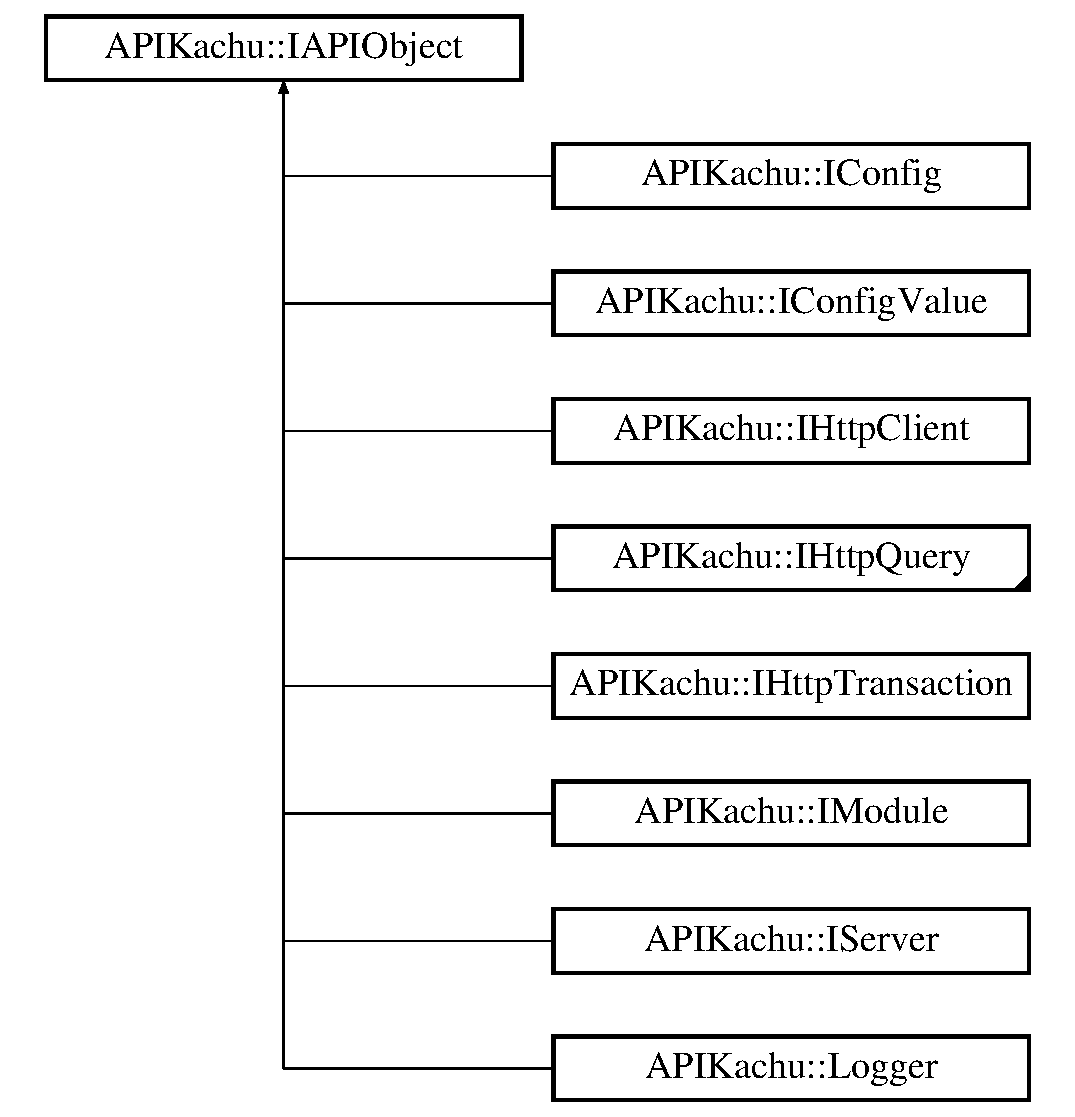
\includegraphics[height=9.000000cm]{class_a_p_i_kachu_1_1_i_a_p_i_object}
\end{center}
\end{figure}
\subsection*{Public Member Functions}
\begin{DoxyCompactItemize}
\item 
virtual uint32 \hyperlink{class_a_p_i_kachu_1_1_i_a_p_i_object_aa7d83f55542775942b2672b6f5db5373}{get\+A\+P\+I\+Magic} () const  =0
\begin{DoxyCompactList}\small\item\em The identifier of the A\+PI. \end{DoxyCompactList}\item 
virtual uint32 \hyperlink{class_a_p_i_kachu_1_1_i_a_p_i_object_aa4517512f286043145854f22671c1f20}{get\+A\+P\+I\+Version} () const  =0
\begin{DoxyCompactList}\small\item\em The version of the A\+PI. \end{DoxyCompactList}\end{DoxyCompactItemize}


\subsection{Detailed Description}
Specifies the A\+PI from which an object comes. 

Interface that covers the entirety of the A\+PI 

\subsection{Member Function Documentation}
\index{A\+P\+I\+Kachu\+::\+I\+A\+P\+I\+Object@{A\+P\+I\+Kachu\+::\+I\+A\+P\+I\+Object}!get\+A\+P\+I\+Magic@{get\+A\+P\+I\+Magic}}
\index{get\+A\+P\+I\+Magic@{get\+A\+P\+I\+Magic}!A\+P\+I\+Kachu\+::\+I\+A\+P\+I\+Object@{A\+P\+I\+Kachu\+::\+I\+A\+P\+I\+Object}}
\subsubsection[{\texorpdfstring{get\+A\+P\+I\+Magic() const  =0}{getAPIMagic() const  =0}}]{\setlength{\rightskip}{0pt plus 5cm}virtual uint32 A\+P\+I\+Kachu\+::\+I\+A\+P\+I\+Object\+::get\+A\+P\+I\+Magic (
\begin{DoxyParamCaption}
{}
\end{DoxyParamCaption}
) const\hspace{0.3cm}{\ttfamily [pure virtual]}}\hypertarget{class_a_p_i_kachu_1_1_i_a_p_i_object_aa7d83f55542775942b2672b6f5db5373}{}\label{class_a_p_i_kachu_1_1_i_a_p_i_object_aa7d83f55542775942b2672b6f5db5373}


The identifier of the A\+PI. 

This should be a unique magic number that identifies your A\+PI so that a module can know which A\+PI an object comes from. Note that this actually using this is not required, but you must still put a unique number here. \index{A\+P\+I\+Kachu\+::\+I\+A\+P\+I\+Object@{A\+P\+I\+Kachu\+::\+I\+A\+P\+I\+Object}!get\+A\+P\+I\+Version@{get\+A\+P\+I\+Version}}
\index{get\+A\+P\+I\+Version@{get\+A\+P\+I\+Version}!A\+P\+I\+Kachu\+::\+I\+A\+P\+I\+Object@{A\+P\+I\+Kachu\+::\+I\+A\+P\+I\+Object}}
\subsubsection[{\texorpdfstring{get\+A\+P\+I\+Version() const  =0}{getAPIVersion() const  =0}}]{\setlength{\rightskip}{0pt plus 5cm}virtual uint32 A\+P\+I\+Kachu\+::\+I\+A\+P\+I\+Object\+::get\+A\+P\+I\+Version (
\begin{DoxyParamCaption}
{}
\end{DoxyParamCaption}
) const\hspace{0.3cm}{\ttfamily [pure virtual]}}\hypertarget{class_a_p_i_kachu_1_1_i_a_p_i_object_aa4517512f286043145854f22671c1f20}{}\label{class_a_p_i_kachu_1_1_i_a_p_i_object_aa4517512f286043145854f22671c1f20}


The version of the A\+PI. 

Complements the magic number with a version of that A\+PI. 

The documentation for this class was generated from the following file\+:\begin{DoxyCompactItemize}
\item 
C\+:/\+Users/\+Mathieu/\+Documents/\+Git\+Hub/\+A\+P\+I-\/\+M\+E\+A\+L/\+A\+P\+I/I\+A\+P\+I\+Object.\+h\end{DoxyCompactItemize}

\hypertarget{class_a_p_i_kachu_1_1_i_config}{}\section{A\+P\+I\+Kachu\+:\+:I\+Config Class Reference}
\label{class_a_p_i_kachu_1_1_i_config}\index{A\+P\+I\+Kachu\+::\+I\+Config@{A\+P\+I\+Kachu\+::\+I\+Config}}


Base interface for the configuration of the server.  




{\ttfamily \#include $<$I\+Config.\+h$>$}

Inheritance diagram for A\+P\+I\+Kachu\+:\+:I\+Config\+:\begin{figure}[H]
\begin{center}
\leavevmode
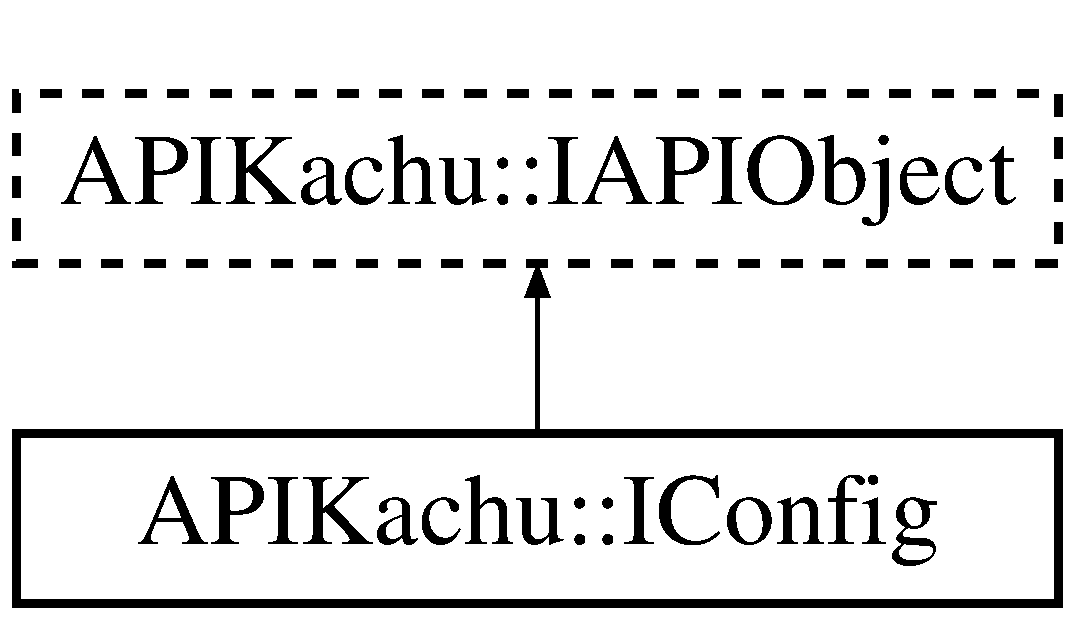
\includegraphics[height=2.000000cm]{class_a_p_i_kachu_1_1_i_config}
\end{center}
\end{figure}
\subsection*{Public Member Functions}
\begin{DoxyCompactItemize}
\item 
virtual bool \hyperlink{class_a_p_i_kachu_1_1_i_config_a117be9b809a9ef2b8bb5ad6834cf2c89}{load} (const std\+::string \&path)=0
\begin{DoxyCompactList}\small\item\em Loads the configuration file. \end{DoxyCompactList}\item 
virtual bool \hyperlink{class_a_p_i_kachu_1_1_i_config_afec3895b88c9f42c1a8e4bf4a79d64cc}{has\+Value} (const std\+::string \&key)=0
\begin{DoxyCompactList}\small\item\em Checks the existence of a value in the configuration file. \end{DoxyCompactList}\item 
virtual const \hyperlink{class_a_p_i_kachu_1_1_i_config_value}{I\+Config\+Value} \& \hyperlink{class_a_p_i_kachu_1_1_i_config_a1dd2e1023713d6720746d0b02de301c8}{get\+Value} (const std\+::string \&key)=0
\begin{DoxyCompactList}\small\item\em Retrieves a value from the configuration file. \end{DoxyCompactList}\end{DoxyCompactItemize}


\subsection{Detailed Description}
Base interface for the configuration of the server. 

\subsection{Member Function Documentation}
\index{A\+P\+I\+Kachu\+::\+I\+Config@{A\+P\+I\+Kachu\+::\+I\+Config}!get\+Value@{get\+Value}}
\index{get\+Value@{get\+Value}!A\+P\+I\+Kachu\+::\+I\+Config@{A\+P\+I\+Kachu\+::\+I\+Config}}
\subsubsection[{\texorpdfstring{get\+Value(const std\+::string \&key)=0}{getValue(const std::string &key)=0}}]{\setlength{\rightskip}{0pt plus 5cm}virtual const {\bf I\+Config\+Value}\& A\+P\+I\+Kachu\+::\+I\+Config\+::get\+Value (
\begin{DoxyParamCaption}
\item[{const std\+::string \&}]{key}
\end{DoxyParamCaption}
)\hspace{0.3cm}{\ttfamily [pure virtual]}}\hypertarget{class_a_p_i_kachu_1_1_i_config_a1dd2e1023713d6720746d0b02de301c8}{}\label{class_a_p_i_kachu_1_1_i_config_a1dd2e1023713d6720746d0b02de301c8}


Retrieves a value from the configuration file. 

Users should always check if the value exists beforehand ; behaviour is undefined otherwise 
\begin{DoxyParams}{Parameters}
{\em std\+::string} & key \\
\hline
\end{DoxyParams}
\index{A\+P\+I\+Kachu\+::\+I\+Config@{A\+P\+I\+Kachu\+::\+I\+Config}!has\+Value@{has\+Value}}
\index{has\+Value@{has\+Value}!A\+P\+I\+Kachu\+::\+I\+Config@{A\+P\+I\+Kachu\+::\+I\+Config}}
\subsubsection[{\texorpdfstring{has\+Value(const std\+::string \&key)=0}{hasValue(const std::string &key)=0}}]{\setlength{\rightskip}{0pt plus 5cm}virtual bool A\+P\+I\+Kachu\+::\+I\+Config\+::has\+Value (
\begin{DoxyParamCaption}
\item[{const std\+::string \&}]{key}
\end{DoxyParamCaption}
)\hspace{0.3cm}{\ttfamily [pure virtual]}}\hypertarget{class_a_p_i_kachu_1_1_i_config_afec3895b88c9f42c1a8e4bf4a79d64cc}{}\label{class_a_p_i_kachu_1_1_i_config_afec3895b88c9f42c1a8e4bf4a79d64cc}


Checks the existence of a value in the configuration file. 

Returns true if the value exists 
\begin{DoxyParams}{Parameters}
{\em std\+::string} & key \\
\hline
\end{DoxyParams}
\index{A\+P\+I\+Kachu\+::\+I\+Config@{A\+P\+I\+Kachu\+::\+I\+Config}!load@{load}}
\index{load@{load}!A\+P\+I\+Kachu\+::\+I\+Config@{A\+P\+I\+Kachu\+::\+I\+Config}}
\subsubsection[{\texorpdfstring{load(const std\+::string \&path)=0}{load(const std::string &path)=0}}]{\setlength{\rightskip}{0pt plus 5cm}virtual bool A\+P\+I\+Kachu\+::\+I\+Config\+::load (
\begin{DoxyParamCaption}
\item[{const std\+::string \&}]{path}
\end{DoxyParamCaption}
)\hspace{0.3cm}{\ttfamily [pure virtual]}}\hypertarget{class_a_p_i_kachu_1_1_i_config_a117be9b809a9ef2b8bb5ad6834cf2c89}{}\label{class_a_p_i_kachu_1_1_i_config_a117be9b809a9ef2b8bb5ad6834cf2c89}


Loads the configuration file. 

Returns true if the loading has succeeded 
\begin{DoxyParams}{Parameters}
{\em std\+::string} & path \\
\hline
\end{DoxyParams}


The documentation for this class was generated from the following file\+:\begin{DoxyCompactItemize}
\item 
C\+:/\+Users/\+Mathieu/\+Documents/\+Git\+Hub/\+A\+P\+I-\/\+M\+E\+A\+L/\+A\+P\+I/I\+Config.\+h\end{DoxyCompactItemize}

\hypertarget{class_a_p_i_kachu_1_1_i_config_value}{}\section{A\+P\+I\+Kachu\+:\+:I\+Config\+Value Class Reference}
\label{class_a_p_i_kachu_1_1_i_config_value}\index{A\+P\+I\+Kachu\+::\+I\+Config\+Value@{A\+P\+I\+Kachu\+::\+I\+Config\+Value}}


Configuration value.  




{\ttfamily \#include $<$I\+Config\+Value.\+h$>$}

Inheritance diagram for A\+P\+I\+Kachu\+:\+:I\+Config\+Value\+:\begin{figure}[H]
\begin{center}
\leavevmode
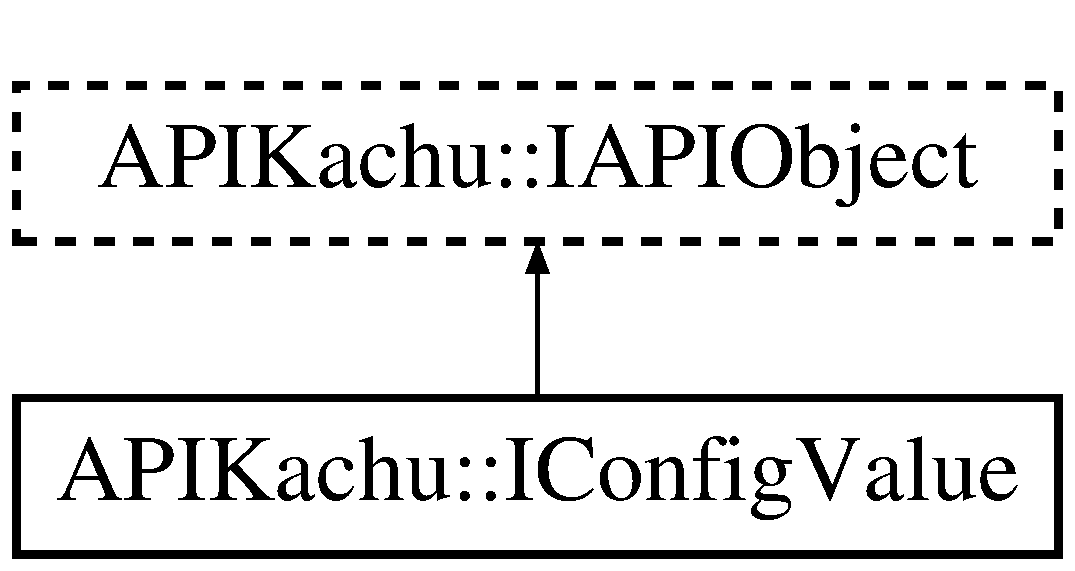
\includegraphics[height=2.000000cm]{class_a_p_i_kachu_1_1_i_config_value}
\end{center}
\end{figure}
\subsection*{Public Member Functions}
\begin{DoxyCompactItemize}
\item 
virtual int8 {\bfseries as\+Int8} () const  =0\hypertarget{class_a_p_i_kachu_1_1_i_config_value_a170f4b3109560e82e8c909d9bc70d942}{}\label{class_a_p_i_kachu_1_1_i_config_value_a170f4b3109560e82e8c909d9bc70d942}

\item 
virtual int16 {\bfseries as\+Int16} () const  =0\hypertarget{class_a_p_i_kachu_1_1_i_config_value_aba1294d7aa777eaecb60510bd91a6644}{}\label{class_a_p_i_kachu_1_1_i_config_value_aba1294d7aa777eaecb60510bd91a6644}

\item 
virtual int32 {\bfseries as\+Int32} () const  =0\hypertarget{class_a_p_i_kachu_1_1_i_config_value_aae8f3229a9cff122ba2dc752bcb65112}{}\label{class_a_p_i_kachu_1_1_i_config_value_aae8f3229a9cff122ba2dc752bcb65112}

\item 
virtual int64 {\bfseries as\+Int64} () const  =0\hypertarget{class_a_p_i_kachu_1_1_i_config_value_a74927e653905be1f9f15994724124917}{}\label{class_a_p_i_kachu_1_1_i_config_value_a74927e653905be1f9f15994724124917}

\item 
virtual uint8 {\bfseries as\+Uint8} () const  =0\hypertarget{class_a_p_i_kachu_1_1_i_config_value_a50063412955139f298da3298f4a70592}{}\label{class_a_p_i_kachu_1_1_i_config_value_a50063412955139f298da3298f4a70592}

\item 
virtual uint16 {\bfseries as\+Uint16} () const  =0\hypertarget{class_a_p_i_kachu_1_1_i_config_value_a76799e2bf46e60655cfe33b51b8fbc15}{}\label{class_a_p_i_kachu_1_1_i_config_value_a76799e2bf46e60655cfe33b51b8fbc15}

\item 
virtual uint32 {\bfseries as\+Uint32} () const  =0\hypertarget{class_a_p_i_kachu_1_1_i_config_value_a61caa2c6d310d4ef4fc96e1cbf70f97f}{}\label{class_a_p_i_kachu_1_1_i_config_value_a61caa2c6d310d4ef4fc96e1cbf70f97f}

\item 
virtual uint64 {\bfseries as\+Uint64} () const  =0\hypertarget{class_a_p_i_kachu_1_1_i_config_value_aa68a9f29da972cbfe9078a097b7febf4}{}\label{class_a_p_i_kachu_1_1_i_config_value_aa68a9f29da972cbfe9078a097b7febf4}

\item 
virtual const std\+::string \& {\bfseries as\+String} () const  =0\hypertarget{class_a_p_i_kachu_1_1_i_config_value_a3ab39fb92e9f1be64e92a672a4bd8632}{}\label{class_a_p_i_kachu_1_1_i_config_value_a3ab39fb92e9f1be64e92a672a4bd8632}

\end{DoxyCompactItemize}


\subsection{Detailed Description}
Configuration value. 

Contains a value and provides conversions to different types 

The documentation for this class was generated from the following file\+:\begin{DoxyCompactItemize}
\item 
C\+:/\+Users/\+Mathieu/\+Documents/\+Git\+Hub/\+A\+P\+I-\/\+M\+E\+A\+L/\+A\+P\+I/I\+Config\+Value.\+h\end{DoxyCompactItemize}

\hypertarget{class_a_p_i_kachu_1_1_i_http_client}{}\section{A\+P\+I\+Kachu\+:\+:I\+Http\+Client Class Reference}
\label{class_a_p_i_kachu_1_1_i_http_client}\index{A\+P\+I\+Kachu\+::\+I\+Http\+Client@{A\+P\+I\+Kachu\+::\+I\+Http\+Client}}


Base interface for a client sending a request.  




{\ttfamily \#include $<$I\+Http\+Client.\+h$>$}

Inheritance diagram for A\+P\+I\+Kachu\+:\+:I\+Http\+Client\+:\begin{figure}[H]
\begin{center}
\leavevmode
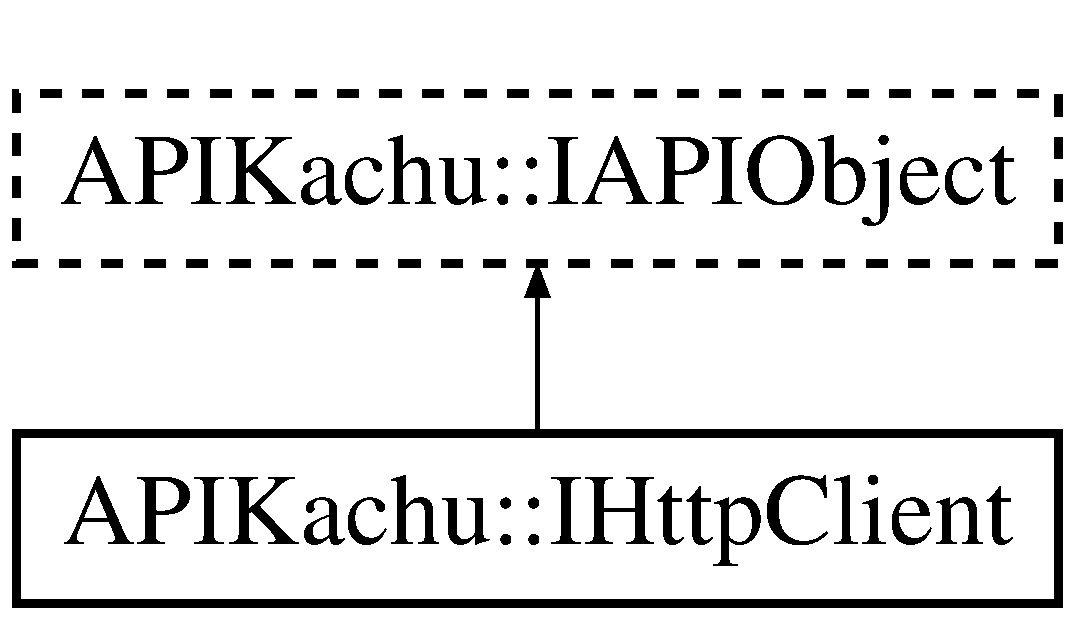
\includegraphics[height=2.000000cm]{class_a_p_i_kachu_1_1_i_http_client}
\end{center}
\end{figure}
\subsection*{Public Member Functions}
\begin{DoxyCompactItemize}
\item 
virtual size\+\_\+t \hyperlink{class_a_p_i_kachu_1_1_i_http_client_a8a6f4cfb1f5cc6b75ba45f707e5aa7bd}{send} (const \hyperlink{class_a_p_i_kachu_1_1_i_http_response}{I\+Http\+Response} \&response)=0
\begin{DoxyCompactList}\small\item\em Sends a response to the client. \end{DoxyCompactList}\item 
virtual const I\+I\+P\+Address \& \hyperlink{class_a_p_i_kachu_1_1_i_http_client_a023c2fcc94ae6757ec1fc0a27cccba1d}{get\+I\+P\+Address} () const  =0\hypertarget{class_a_p_i_kachu_1_1_i_http_client_a023c2fcc94ae6757ec1fc0a27cccba1d}{}\label{class_a_p_i_kachu_1_1_i_http_client_a023c2fcc94ae6757ec1fc0a27cccba1d}

\begin{DoxyCompactList}\small\item\em Getter for the IP address. \end{DoxyCompactList}\end{DoxyCompactItemize}


\subsection{Detailed Description}
Base interface for a client sending a request. 

\subsection{Member Function Documentation}
\index{A\+P\+I\+Kachu\+::\+I\+Http\+Client@{A\+P\+I\+Kachu\+::\+I\+Http\+Client}!send@{send}}
\index{send@{send}!A\+P\+I\+Kachu\+::\+I\+Http\+Client@{A\+P\+I\+Kachu\+::\+I\+Http\+Client}}
\subsubsection[{\texorpdfstring{send(const I\+Http\+Response \&response)=0}{send(const IHttpResponse &response)=0}}]{\setlength{\rightskip}{0pt plus 5cm}virtual size\+\_\+t A\+P\+I\+Kachu\+::\+I\+Http\+Client\+::send (
\begin{DoxyParamCaption}
\item[{const {\bf I\+Http\+Response} \&}]{response}
\end{DoxyParamCaption}
)\hspace{0.3cm}{\ttfamily [pure virtual]}}\hypertarget{class_a_p_i_kachu_1_1_i_http_client_a8a6f4cfb1f5cc6b75ba45f707e5aa7bd}{}\label{class_a_p_i_kachu_1_1_i_http_client_a8a6f4cfb1f5cc6b75ba45f707e5aa7bd}


Sends a response to the client. 

Returns -\/1 on error or the number of bytes sent 
\begin{DoxyParams}{Parameters}
{\em const} & \hyperlink{class_a_p_i_kachu_1_1_i_http_response}{I\+Http\+Response} \&response -\/ the response to be sent \\
\hline
\end{DoxyParams}


The documentation for this class was generated from the following file\+:\begin{DoxyCompactItemize}
\item 
C\+:/\+Users/\+Mathieu/\+Documents/\+Git\+Hub/\+A\+P\+I-\/\+M\+E\+A\+L/\+A\+P\+I/I\+Http\+Client.\+h\end{DoxyCompactItemize}

\hypertarget{class_a_p_i_kachu_1_1_i_http_query}{}\section{A\+P\+I\+Kachu\+:\+:I\+Http\+Query Class Reference}
\label{class_a_p_i_kachu_1_1_i_http_query}\index{A\+P\+I\+Kachu\+::\+I\+Http\+Query@{A\+P\+I\+Kachu\+::\+I\+Http\+Query}}


Base class for an H\+T\+TP query.  




{\ttfamily \#include $<$I\+Http\+Query.\+h$>$}

Inheritance diagram for A\+P\+I\+Kachu\+:\+:I\+Http\+Query\+:\begin{figure}[H]
\begin{center}
\leavevmode
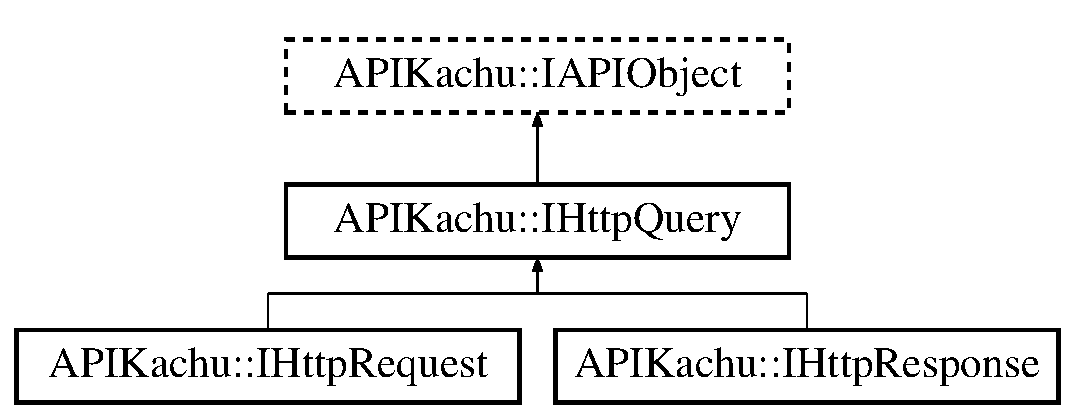
\includegraphics[height=3.000000cm]{class_a_p_i_kachu_1_1_i_http_query}
\end{center}
\end{figure}
\subsection*{Public Types}
\begin{DoxyCompactItemize}
\item 
typedef std\+::map$<$ std\+::string, std\+::string $>$ \hyperlink{class_a_p_i_kachu_1_1_i_http_query_a15c3c9bc16ea76d23181bdc95e3ecca7}{t\+Headers}
\begin{DoxyCompactList}\small\item\em Associative container for http headers. \end{DoxyCompactList}\end{DoxyCompactItemize}
\subsection*{Public Member Functions}
\begin{DoxyCompactItemize}
\item 
virtual const \hyperlink{class_a_p_i_kachu_1_1_i_http_query_a15c3c9bc16ea76d23181bdc95e3ecca7}{t\+Headers} \& \hyperlink{class_a_p_i_kachu_1_1_i_http_query_ad7181b39532a572f26f3ed23e3b8aa4b}{get\+Headers} () const  =0
\begin{DoxyCompactList}\small\item\em Getter for the http headers. \end{DoxyCompactList}\item 
virtual const \hyperlink{struct_a_p_i_kachu_1_1_byte_buffer}{Byte\+Buffer} \& \hyperlink{class_a_p_i_kachu_1_1_i_http_query_a0125257a775e3652c170d2f5b35f62d7}{get\+Byte\+Buffer} () const  =0
\begin{DoxyCompactList}\small\item\em Getter for the content of the query. \end{DoxyCompactList}\item 
virtual \hyperlink{struct_a_p_i_kachu_1_1_byte_buffer}{Byte\+Buffer} \& \hyperlink{class_a_p_i_kachu_1_1_i_http_query_ab2e6857af2e0fcf8b80d19efff89c971}{get\+Byte\+Buffer} ()=0
\begin{DoxyCompactList}\small\item\em Getter for the content of the query. \end{DoxyCompactList}\item 
virtual const std\+::string \& \hyperlink{class_a_p_i_kachu_1_1_i_http_query_afcb8d29d65a39d58aeec117aebbeb210}{get\+H\+T\+T\+P\+Version} () const  =0\hypertarget{class_a_p_i_kachu_1_1_i_http_query_afcb8d29d65a39d58aeec117aebbeb210}{}\label{class_a_p_i_kachu_1_1_i_http_query_afcb8d29d65a39d58aeec117aebbeb210}

\begin{DoxyCompactList}\small\item\em Getter for the http version of the query. \end{DoxyCompactList}\end{DoxyCompactItemize}


\subsection{Detailed Description}
Base class for an H\+T\+TP query. 

Inherited by \hyperlink{class_a_p_i_kachu_1_1_i_http_response}{I\+Http\+Response} and \hyperlink{class_a_p_i_kachu_1_1_i_http_request}{I\+Http\+Request} 

\subsection{Member Typedef Documentation}
\index{A\+P\+I\+Kachu\+::\+I\+Http\+Query@{A\+P\+I\+Kachu\+::\+I\+Http\+Query}!t\+Headers@{t\+Headers}}
\index{t\+Headers@{t\+Headers}!A\+P\+I\+Kachu\+::\+I\+Http\+Query@{A\+P\+I\+Kachu\+::\+I\+Http\+Query}}
\subsubsection[{\texorpdfstring{t\+Headers}{tHeaders}}]{\setlength{\rightskip}{0pt plus 5cm}typedef std\+::map$<$std\+::string, std\+::string$>$ {\bf A\+P\+I\+Kachu\+::\+I\+Http\+Query\+::t\+Headers}}\hypertarget{class_a_p_i_kachu_1_1_i_http_query_a15c3c9bc16ea76d23181bdc95e3ecca7}{}\label{class_a_p_i_kachu_1_1_i_http_query_a15c3c9bc16ea76d23181bdc95e3ecca7}


Associative container for http headers. 

Key and values are strings 

\subsection{Member Function Documentation}
\index{A\+P\+I\+Kachu\+::\+I\+Http\+Query@{A\+P\+I\+Kachu\+::\+I\+Http\+Query}!get\+Byte\+Buffer@{get\+Byte\+Buffer}}
\index{get\+Byte\+Buffer@{get\+Byte\+Buffer}!A\+P\+I\+Kachu\+::\+I\+Http\+Query@{A\+P\+I\+Kachu\+::\+I\+Http\+Query}}
\subsubsection[{\texorpdfstring{get\+Byte\+Buffer() const  =0}{getByteBuffer() const  =0}}]{\setlength{\rightskip}{0pt plus 5cm}virtual const {\bf Byte\+Buffer}\& A\+P\+I\+Kachu\+::\+I\+Http\+Query\+::get\+Byte\+Buffer (
\begin{DoxyParamCaption}
{}
\end{DoxyParamCaption}
) const\hspace{0.3cm}{\ttfamily [pure virtual]}}\hypertarget{class_a_p_i_kachu_1_1_i_http_query_a0125257a775e3652c170d2f5b35f62d7}{}\label{class_a_p_i_kachu_1_1_i_http_query_a0125257a775e3652c170d2f5b35f62d7}


Getter for the content of the query. 

See documentation for \hyperlink{struct_a_p_i_kachu_1_1_byte_buffer}{Byte\+Buffer} \index{A\+P\+I\+Kachu\+::\+I\+Http\+Query@{A\+P\+I\+Kachu\+::\+I\+Http\+Query}!get\+Byte\+Buffer@{get\+Byte\+Buffer}}
\index{get\+Byte\+Buffer@{get\+Byte\+Buffer}!A\+P\+I\+Kachu\+::\+I\+Http\+Query@{A\+P\+I\+Kachu\+::\+I\+Http\+Query}}
\subsubsection[{\texorpdfstring{get\+Byte\+Buffer()=0}{getByteBuffer()=0}}]{\setlength{\rightskip}{0pt plus 5cm}virtual {\bf Byte\+Buffer}\& A\+P\+I\+Kachu\+::\+I\+Http\+Query\+::get\+Byte\+Buffer (
\begin{DoxyParamCaption}
{}
\end{DoxyParamCaption}
)\hspace{0.3cm}{\ttfamily [pure virtual]}}\hypertarget{class_a_p_i_kachu_1_1_i_http_query_ab2e6857af2e0fcf8b80d19efff89c971}{}\label{class_a_p_i_kachu_1_1_i_http_query_ab2e6857af2e0fcf8b80d19efff89c971}


Getter for the content of the query. 

See documentation for \hyperlink{struct_a_p_i_kachu_1_1_byte_buffer}{Byte\+Buffer} \index{A\+P\+I\+Kachu\+::\+I\+Http\+Query@{A\+P\+I\+Kachu\+::\+I\+Http\+Query}!get\+Headers@{get\+Headers}}
\index{get\+Headers@{get\+Headers}!A\+P\+I\+Kachu\+::\+I\+Http\+Query@{A\+P\+I\+Kachu\+::\+I\+Http\+Query}}
\subsubsection[{\texorpdfstring{get\+Headers() const  =0}{getHeaders() const  =0}}]{\setlength{\rightskip}{0pt plus 5cm}virtual const {\bf t\+Headers}\& A\+P\+I\+Kachu\+::\+I\+Http\+Query\+::get\+Headers (
\begin{DoxyParamCaption}
{}
\end{DoxyParamCaption}
) const\hspace{0.3cm}{\ttfamily [pure virtual]}}\hypertarget{class_a_p_i_kachu_1_1_i_http_query_ad7181b39532a572f26f3ed23e3b8aa4b}{}\label{class_a_p_i_kachu_1_1_i_http_query_ad7181b39532a572f26f3ed23e3b8aa4b}


Getter for the http headers. 

See documentation for t\+Headers 

The documentation for this class was generated from the following file\+:\begin{DoxyCompactItemize}
\item 
C\+:/\+Users/\+Mathieu/\+Documents/\+Git\+Hub/\+A\+P\+I-\/\+M\+E\+A\+L/\+A\+P\+I/I\+Http\+Query.\+h\end{DoxyCompactItemize}

\hypertarget{class_a_p_i_kachu_1_1_i_http_request}{}\section{A\+P\+I\+Kachu\+:\+:I\+Http\+Request Class Reference}
\label{class_a_p_i_kachu_1_1_i_http_request}\index{A\+P\+I\+Kachu\+::\+I\+Http\+Request@{A\+P\+I\+Kachu\+::\+I\+Http\+Request}}


Contains a request sent by a client.  




{\ttfamily \#include $<$I\+Http\+Request.\+h$>$}

Inheritance diagram for A\+P\+I\+Kachu\+:\+:I\+Http\+Request\+:\begin{figure}[H]
\begin{center}
\leavevmode
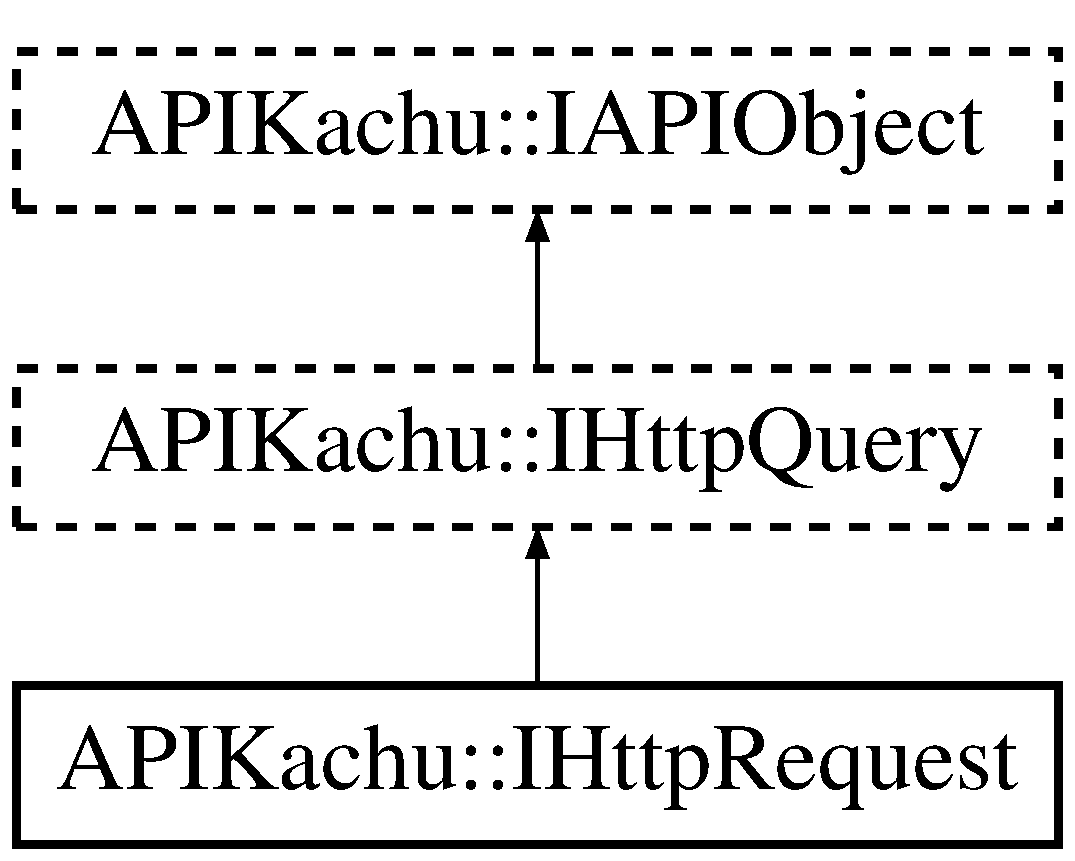
\includegraphics[height=3.000000cm]{class_a_p_i_kachu_1_1_i_http_request}
\end{center}
\end{figure}
\subsection*{Public Member Functions}
\begin{DoxyCompactItemize}
\item 
virtual \hyperlink{namespace_a_p_i_kachu_aeff09045bb4c289dc6f23d46950d830e}{e\+Http\+Method} \hyperlink{class_a_p_i_kachu_1_1_i_http_request_a95846739542dcccdd6cb8241192be350}{get\+Method} () const  =0
\begin{DoxyCompactList}\small\item\em Getter for the http method of the request. \end{DoxyCompactList}\item 
virtual const std\+::string \& \hyperlink{class_a_p_i_kachu_1_1_i_http_request_a32e5c6e709b6f753597f1364beb9e6c4}{get\+U\+RN} () const  =0\hypertarget{class_a_p_i_kachu_1_1_i_http_request_a32e5c6e709b6f753597f1364beb9e6c4}{}\label{class_a_p_i_kachu_1_1_i_http_request_a32e5c6e709b6f753597f1364beb9e6c4}

\begin{DoxyCompactList}\small\item\em Getter for the U\+RN of the request. \end{DoxyCompactList}\end{DoxyCompactItemize}
\subsection*{Additional Inherited Members}


\subsection{Detailed Description}
Contains a request sent by a client. 

Inherits \hyperlink{class_a_p_i_kachu_1_1_i_http_query}{I\+Http\+Query} 

\subsection{Member Function Documentation}
\index{A\+P\+I\+Kachu\+::\+I\+Http\+Request@{A\+P\+I\+Kachu\+::\+I\+Http\+Request}!get\+Method@{get\+Method}}
\index{get\+Method@{get\+Method}!A\+P\+I\+Kachu\+::\+I\+Http\+Request@{A\+P\+I\+Kachu\+::\+I\+Http\+Request}}
\subsubsection[{\texorpdfstring{get\+Method() const  =0}{getMethod() const  =0}}]{\setlength{\rightskip}{0pt plus 5cm}virtual {\bf e\+Http\+Method} A\+P\+I\+Kachu\+::\+I\+Http\+Request\+::get\+Method (
\begin{DoxyParamCaption}
{}
\end{DoxyParamCaption}
) const\hspace{0.3cm}{\ttfamily [pure virtual]}}\hypertarget{class_a_p_i_kachu_1_1_i_http_request_a95846739542dcccdd6cb8241192be350}{}\label{class_a_p_i_kachu_1_1_i_http_request_a95846739542dcccdd6cb8241192be350}


Getter for the http method of the request. 

See documentation for e\+Http\+Method 

The documentation for this class was generated from the following file\+:\begin{DoxyCompactItemize}
\item 
C\+:/\+Users/\+Mathieu/\+Documents/\+Git\+Hub/\+A\+P\+I-\/\+M\+E\+A\+L/\+A\+P\+I/I\+Http\+Request.\+h\end{DoxyCompactItemize}

\hypertarget{class_a_p_i_kachu_1_1_i_http_response}{}\section{A\+P\+I\+Kachu\+:\+:I\+Http\+Response Class Reference}
\label{class_a_p_i_kachu_1_1_i_http_response}\index{A\+P\+I\+Kachu\+::\+I\+Http\+Response@{A\+P\+I\+Kachu\+::\+I\+Http\+Response}}


Contains a response to be sent to a client.  




{\ttfamily \#include $<$I\+Http\+Response.\+h$>$}

Inheritance diagram for A\+P\+I\+Kachu\+:\+:I\+Http\+Response\+:\begin{figure}[H]
\begin{center}
\leavevmode
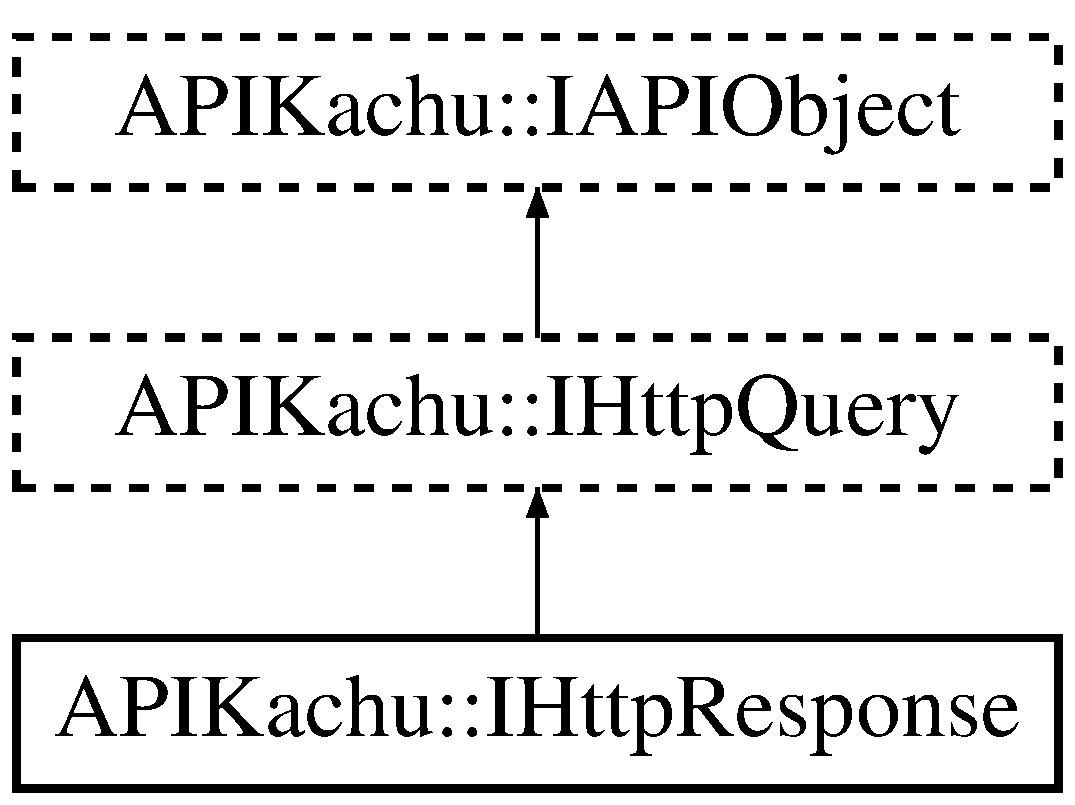
\includegraphics[height=3.000000cm]{class_a_p_i_kachu_1_1_i_http_response}
\end{center}
\end{figure}
\subsection*{Public Member Functions}
\begin{DoxyCompactItemize}
\item 
virtual void \hyperlink{class_a_p_i_kachu_1_1_i_http_response_a9ade9f1dda4f365140c71699b7b15d7d}{set\+Status} (uint16 status)=0
\begin{DoxyCompactList}\small\item\em Setter for the status code of the response. \end{DoxyCompactList}\item 
virtual uint16 \hyperlink{class_a_p_i_kachu_1_1_i_http_response_a1f4ff13d6f6d85d216777c7c88dc0d29}{get\+Status} () const  =0
\begin{DoxyCompactList}\small\item\em Getter for the status code of the response. \end{DoxyCompactList}\end{DoxyCompactItemize}
\subsection*{Additional Inherited Members}


\subsection{Detailed Description}
Contains a response to be sent to a client. 

Inherits \hyperlink{class_a_p_i_kachu_1_1_i_http_query}{I\+Http\+Query} 

\subsection{Member Function Documentation}
\index{A\+P\+I\+Kachu\+::\+I\+Http\+Response@{A\+P\+I\+Kachu\+::\+I\+Http\+Response}!get\+Status@{get\+Status}}
\index{get\+Status@{get\+Status}!A\+P\+I\+Kachu\+::\+I\+Http\+Response@{A\+P\+I\+Kachu\+::\+I\+Http\+Response}}
\subsubsection[{\texorpdfstring{get\+Status() const  =0}{getStatus() const  =0}}]{\setlength{\rightskip}{0pt plus 5cm}virtual uint16 A\+P\+I\+Kachu\+::\+I\+Http\+Response\+::get\+Status (
\begin{DoxyParamCaption}
{}
\end{DoxyParamCaption}
) const\hspace{0.3cm}{\ttfamily [pure virtual]}}\hypertarget{class_a_p_i_kachu_1_1_i_http_response_a1f4ff13d6f6d85d216777c7c88dc0d29}{}\label{class_a_p_i_kachu_1_1_i_http_response_a1f4ff13d6f6d85d216777c7c88dc0d29}


Getter for the status code of the response. 

\begin{DoxyReturn}{Returns}
uint16 
\end{DoxyReturn}
\index{A\+P\+I\+Kachu\+::\+I\+Http\+Response@{A\+P\+I\+Kachu\+::\+I\+Http\+Response}!set\+Status@{set\+Status}}
\index{set\+Status@{set\+Status}!A\+P\+I\+Kachu\+::\+I\+Http\+Response@{A\+P\+I\+Kachu\+::\+I\+Http\+Response}}
\subsubsection[{\texorpdfstring{set\+Status(uint16 status)=0}{setStatus(uint16 status)=0}}]{\setlength{\rightskip}{0pt plus 5cm}virtual void A\+P\+I\+Kachu\+::\+I\+Http\+Response\+::set\+Status (
\begin{DoxyParamCaption}
\item[{uint16}]{status}
\end{DoxyParamCaption}
)\hspace{0.3cm}{\ttfamily [pure virtual]}}\hypertarget{class_a_p_i_kachu_1_1_i_http_response_a9ade9f1dda4f365140c71699b7b15d7d}{}\label{class_a_p_i_kachu_1_1_i_http_response_a9ade9f1dda4f365140c71699b7b15d7d}


Setter for the status code of the response. 


\begin{DoxyParams}{Parameters}
{\em uint16} & status \\
\hline
\end{DoxyParams}


The documentation for this class was generated from the following file\+:\begin{DoxyCompactItemize}
\item 
Documents/bite/\+A\+P\+I-\/\+K\+A\+C\+H\+U/\+A\+P\+I/I\+Http\+Response.\+h\end{DoxyCompactItemize}

\hypertarget{class_a_p_i_kachu_1_1_i_http_transaction}{}\section{A\+P\+I\+Kachu\+:\+:I\+Http\+Transaction Class Reference}
\label{class_a_p_i_kachu_1_1_i_http_transaction}\index{A\+P\+I\+Kachu\+::\+I\+Http\+Transaction@{A\+P\+I\+Kachu\+::\+I\+Http\+Transaction}}


Class containing informations about an H\+T\+TP transaction.  




{\ttfamily \#include $<$I\+Http\+Transaction.\+h$>$}

Inheritance diagram for A\+P\+I\+Kachu\+:\+:I\+Http\+Transaction\+:\begin{figure}[H]
\begin{center}
\leavevmode
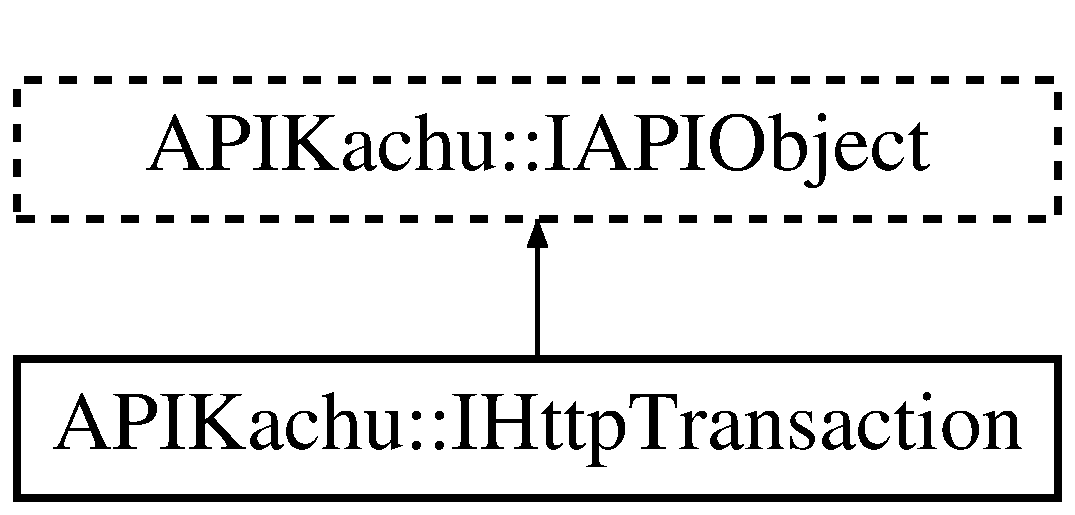
\includegraphics[height=2.000000cm]{class_a_p_i_kachu_1_1_i_http_transaction}
\end{center}
\end{figure}
\subsection*{Public Member Functions}
\begin{DoxyCompactItemize}
\item 
virtual void \hyperlink{class_a_p_i_kachu_1_1_i_http_transaction_a4d764f4e4e7e6a9f977cb849e56f9540}{set\+Http\+Request} (\hyperlink{class_a_p_i_kachu_1_1_i_http_request}{I\+Http\+Request} $\ast$request)=0
\begin{DoxyCompactList}\small\item\em Setter for the http request. \end{DoxyCompactList}\item 
virtual void \hyperlink{class_a_p_i_kachu_1_1_i_http_transaction_a42505225ef609ed6b2809b740fb1a057}{set\+Http\+Response} (\hyperlink{class_a_p_i_kachu_1_1_i_http_response}{I\+Http\+Response} $\ast$response)=0
\begin{DoxyCompactList}\small\item\em Setter for the http response. \end{DoxyCompactList}\item 
virtual \hyperlink{class_a_p_i_kachu_1_1_i_http_client}{I\+Http\+Client} $\ast$ \hyperlink{class_a_p_i_kachu_1_1_i_http_transaction_a5c36ff3eb4eda6cd2c981a7f595fe26f}{get\+Http\+Client} ()=0
\begin{DoxyCompactList}\small\item\em Getter for the client sending the request. \end{DoxyCompactList}\item 
virtual \hyperlink{class_a_p_i_kachu_1_1_i_http_request}{I\+Http\+Request} $\ast$ \hyperlink{class_a_p_i_kachu_1_1_i_http_transaction_a6e2cac980600fc7ac2f7d13c366e5e0a}{get\+Http\+Request} ()=0
\begin{DoxyCompactList}\small\item\em Getter for the http request of the transaction. \end{DoxyCompactList}\item 
virtual \hyperlink{class_a_p_i_kachu_1_1_i_http_response}{I\+Http\+Response} $\ast$ \hyperlink{class_a_p_i_kachu_1_1_i_http_transaction_a12da5989c6c9417c7c4b80e02345937c}{get\+Http\+Response} ()=0
\begin{DoxyCompactList}\small\item\em Getter for the http response of the transaction. \end{DoxyCompactList}\item 
virtual const \hyperlink{struct_a_p_i_kachu_1_1_byte_buffer}{Byte\+Buffer} \& \hyperlink{class_a_p_i_kachu_1_1_i_http_transaction_a83b2b8c2fc400512de18a996bae835ae}{get\+Raw\+Request} ()=0
\begin{DoxyCompactList}\small\item\em Getter for the raw data of the received packet. \end{DoxyCompactList}\end{DoxyCompactItemize}


\subsection{Detailed Description}
Class containing informations about an H\+T\+TP transaction. 

Defines the request, the client sending it, and the response built by the server 

\subsection{Member Function Documentation}
\index{A\+P\+I\+Kachu\+::\+I\+Http\+Transaction@{A\+P\+I\+Kachu\+::\+I\+Http\+Transaction}!get\+Http\+Client@{get\+Http\+Client}}
\index{get\+Http\+Client@{get\+Http\+Client}!A\+P\+I\+Kachu\+::\+I\+Http\+Transaction@{A\+P\+I\+Kachu\+::\+I\+Http\+Transaction}}
\subsubsection[{\texorpdfstring{get\+Http\+Client()=0}{getHttpClient()=0}}]{\setlength{\rightskip}{0pt plus 5cm}virtual {\bf I\+Http\+Client}$\ast$ A\+P\+I\+Kachu\+::\+I\+Http\+Transaction\+::get\+Http\+Client (
\begin{DoxyParamCaption}
{}
\end{DoxyParamCaption}
)\hspace{0.3cm}{\ttfamily [pure virtual]}}\hypertarget{class_a_p_i_kachu_1_1_i_http_transaction_a5c36ff3eb4eda6cd2c981a7f595fe26f}{}\label{class_a_p_i_kachu_1_1_i_http_transaction_a5c36ff3eb4eda6cd2c981a7f595fe26f}


Getter for the client sending the request. 

This should be set by the server upon receiving a packet \index{A\+P\+I\+Kachu\+::\+I\+Http\+Transaction@{A\+P\+I\+Kachu\+::\+I\+Http\+Transaction}!get\+Http\+Request@{get\+Http\+Request}}
\index{get\+Http\+Request@{get\+Http\+Request}!A\+P\+I\+Kachu\+::\+I\+Http\+Transaction@{A\+P\+I\+Kachu\+::\+I\+Http\+Transaction}}
\subsubsection[{\texorpdfstring{get\+Http\+Request()=0}{getHttpRequest()=0}}]{\setlength{\rightskip}{0pt plus 5cm}virtual {\bf I\+Http\+Request}$\ast$ A\+P\+I\+Kachu\+::\+I\+Http\+Transaction\+::get\+Http\+Request (
\begin{DoxyParamCaption}
{}
\end{DoxyParamCaption}
)\hspace{0.3cm}{\ttfamily [pure virtual]}}\hypertarget{class_a_p_i_kachu_1_1_i_http_transaction_a6e2cac980600fc7ac2f7d13c366e5e0a}{}\label{class_a_p_i_kachu_1_1_i_http_transaction_a6e2cac980600fc7ac2f7d13c366e5e0a}


Getter for the http request of the transaction. 

Returns nullptr if the request has not been parsed yet \index{A\+P\+I\+Kachu\+::\+I\+Http\+Transaction@{A\+P\+I\+Kachu\+::\+I\+Http\+Transaction}!get\+Http\+Response@{get\+Http\+Response}}
\index{get\+Http\+Response@{get\+Http\+Response}!A\+P\+I\+Kachu\+::\+I\+Http\+Transaction@{A\+P\+I\+Kachu\+::\+I\+Http\+Transaction}}
\subsubsection[{\texorpdfstring{get\+Http\+Response()=0}{getHttpResponse()=0}}]{\setlength{\rightskip}{0pt plus 5cm}virtual {\bf I\+Http\+Response}$\ast$ A\+P\+I\+Kachu\+::\+I\+Http\+Transaction\+::get\+Http\+Response (
\begin{DoxyParamCaption}
{}
\end{DoxyParamCaption}
)\hspace{0.3cm}{\ttfamily [pure virtual]}}\hypertarget{class_a_p_i_kachu_1_1_i_http_transaction_a12da5989c6c9417c7c4b80e02345937c}{}\label{class_a_p_i_kachu_1_1_i_http_transaction_a12da5989c6c9417c7c4b80e02345937c}


Getter for the http response of the transaction. 

Returns nullptr if the response has not been built yet \index{A\+P\+I\+Kachu\+::\+I\+Http\+Transaction@{A\+P\+I\+Kachu\+::\+I\+Http\+Transaction}!get\+Raw\+Request@{get\+Raw\+Request}}
\index{get\+Raw\+Request@{get\+Raw\+Request}!A\+P\+I\+Kachu\+::\+I\+Http\+Transaction@{A\+P\+I\+Kachu\+::\+I\+Http\+Transaction}}
\subsubsection[{\texorpdfstring{get\+Raw\+Request()=0}{getRawRequest()=0}}]{\setlength{\rightskip}{0pt plus 5cm}virtual const {\bf Byte\+Buffer}\& A\+P\+I\+Kachu\+::\+I\+Http\+Transaction\+::get\+Raw\+Request (
\begin{DoxyParamCaption}
{}
\end{DoxyParamCaption}
)\hspace{0.3cm}{\ttfamily [pure virtual]}}\hypertarget{class_a_p_i_kachu_1_1_i_http_transaction_a83b2b8c2fc400512de18a996bae835ae}{}\label{class_a_p_i_kachu_1_1_i_http_transaction_a83b2b8c2fc400512de18a996bae835ae}


Getter for the raw data of the received packet. 

Should be set by the server upon receiving a packet

See documentation for \hyperlink{struct_a_p_i_kachu_1_1_byte_buffer}{Byte\+Buffer} \index{A\+P\+I\+Kachu\+::\+I\+Http\+Transaction@{A\+P\+I\+Kachu\+::\+I\+Http\+Transaction}!set\+Http\+Request@{set\+Http\+Request}}
\index{set\+Http\+Request@{set\+Http\+Request}!A\+P\+I\+Kachu\+::\+I\+Http\+Transaction@{A\+P\+I\+Kachu\+::\+I\+Http\+Transaction}}
\subsubsection[{\texorpdfstring{set\+Http\+Request(\+I\+Http\+Request $\ast$request)=0}{setHttpRequest(IHttpRequest *request)=0}}]{\setlength{\rightskip}{0pt plus 5cm}virtual void A\+P\+I\+Kachu\+::\+I\+Http\+Transaction\+::set\+Http\+Request (
\begin{DoxyParamCaption}
\item[{{\bf I\+Http\+Request} $\ast$}]{request}
\end{DoxyParamCaption}
)\hspace{0.3cm}{\ttfamily [pure virtual]}}\hypertarget{class_a_p_i_kachu_1_1_i_http_transaction_a4d764f4e4e7e6a9f977cb849e56f9540}{}\label{class_a_p_i_kachu_1_1_i_http_transaction_a4d764f4e4e7e6a9f977cb849e56f9540}


Setter for the http request. 

Should be used by the first module when parsing the request 
\begin{DoxyParams}{Parameters}
{\em \hyperlink{class_a_p_i_kachu_1_1_i_http_request}{I\+Http\+Request}} & $\ast$request \\
\hline
\end{DoxyParams}
\index{A\+P\+I\+Kachu\+::\+I\+Http\+Transaction@{A\+P\+I\+Kachu\+::\+I\+Http\+Transaction}!set\+Http\+Response@{set\+Http\+Response}}
\index{set\+Http\+Response@{set\+Http\+Response}!A\+P\+I\+Kachu\+::\+I\+Http\+Transaction@{A\+P\+I\+Kachu\+::\+I\+Http\+Transaction}}
\subsubsection[{\texorpdfstring{set\+Http\+Response(\+I\+Http\+Response $\ast$response)=0}{setHttpResponse(IHttpResponse *response)=0}}]{\setlength{\rightskip}{0pt plus 5cm}virtual void A\+P\+I\+Kachu\+::\+I\+Http\+Transaction\+::set\+Http\+Response (
\begin{DoxyParamCaption}
\item[{{\bf I\+Http\+Response} $\ast$}]{response}
\end{DoxyParamCaption}
)\hspace{0.3cm}{\ttfamily [pure virtual]}}\hypertarget{class_a_p_i_kachu_1_1_i_http_transaction_a42505225ef609ed6b2809b740fb1a057}{}\label{class_a_p_i_kachu_1_1_i_http_transaction_a42505225ef609ed6b2809b740fb1a057}


Setter for the http response. 

Should be used by the first module when building the response 
\begin{DoxyParams}{Parameters}
{\em \hyperlink{class_a_p_i_kachu_1_1_i_http_response}{I\+Http\+Response}} & $\ast$response \\
\hline
\end{DoxyParams}


The documentation for this class was generated from the following file\+:\begin{DoxyCompactItemize}
\item 
Documents/bite/\+A\+P\+I-\/\+K\+A\+C\+H\+U/\+A\+P\+I/I\+Http\+Transaction.\+h\end{DoxyCompactItemize}

\hypertarget{class_a_p_i_kachu_1_1_i_module}{}\section{A\+P\+I\+Kachu\+:\+:I\+Module Class Reference}
\label{class_a_p_i_kachu_1_1_i_module}\index{A\+P\+I\+Kachu\+::\+I\+Module@{A\+P\+I\+Kachu\+::\+I\+Module}}


Base interface for a module.  




{\ttfamily \#include $<$I\+Module.\+h$>$}

Inheritance diagram for A\+P\+I\+Kachu\+:\+:I\+Module\+:\begin{figure}[H]
\begin{center}
\leavevmode
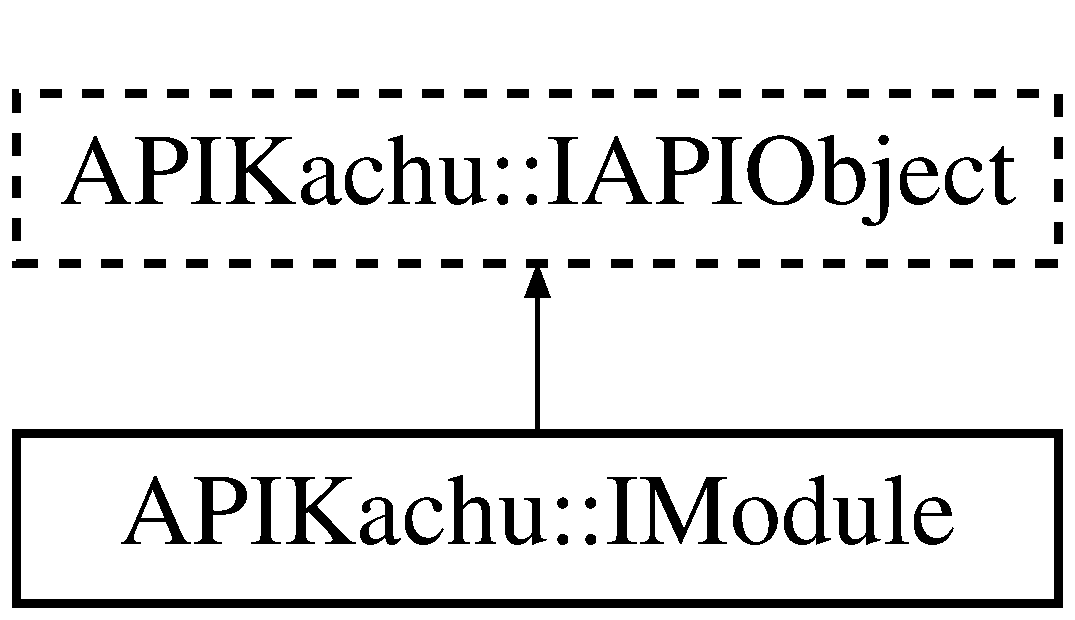
\includegraphics[height=2.000000cm]{class_a_p_i_kachu_1_1_i_module}
\end{center}
\end{figure}
\subsection*{Public Member Functions}
\begin{DoxyCompactItemize}
\item 
virtual bool \hyperlink{class_a_p_i_kachu_1_1_i_module_a594205683c6dd0af322d15d2d4557ea7}{exec} (\hyperlink{class_a_p_i_kachu_1_1_i_http_transaction}{I\+Http\+Transaction} $\ast$)=0
\begin{DoxyCompactList}\small\item\em Method to be used by the server on each H\+T\+TP query received. \end{DoxyCompactList}\item 
virtual bool \hyperlink{class_a_p_i_kachu_1_1_i_module_a7dbb157b5dd00111c9164b9fa078e151}{init} (\hyperlink{class_a_p_i_kachu_1_1_i_server}{I\+Server} $\ast$)=0
\begin{DoxyCompactList}\small\item\em Method to be used when the server is started. \end{DoxyCompactList}\item 
virtual uint8 \hyperlink{class_a_p_i_kachu_1_1_i_module_abd348ba61de8854ba4c9cf0d3b19541c}{get\+Module\+Type} () const  =0
\begin{DoxyCompactList}\small\item\em Getter for the module\textquotesingle{}s type. \end{DoxyCompactList}\item 
virtual uint8 \hyperlink{class_a_p_i_kachu_1_1_i_module_ad0ec3789fb8afa922937f8e95db8badf}{get\+Module\+Flags} () const  =0
\begin{DoxyCompactList}\small\item\em Getter for the module\textquotesingle{}s flags. \end{DoxyCompactList}\item 
virtual uint8 \hyperlink{class_a_p_i_kachu_1_1_i_module_aaad7d8817c8b1344fbe310d7e5e85404}{get\+Handled\+Methods} () const  =0
\begin{DoxyCompactList}\small\item\em Getter for the module\textquotesingle{}s handled methods. \end{DoxyCompactList}\end{DoxyCompactItemize}


\subsection{Detailed Description}
Base interface for a module. 

Implements the basic methods to be used by the server 

\subsection{Member Function Documentation}
\index{A\+P\+I\+Kachu\+::\+I\+Module@{A\+P\+I\+Kachu\+::\+I\+Module}!exec@{exec}}
\index{exec@{exec}!A\+P\+I\+Kachu\+::\+I\+Module@{A\+P\+I\+Kachu\+::\+I\+Module}}
\subsubsection[{\texorpdfstring{exec(\+I\+Http\+Transaction $\ast$)=0}{exec(IHttpTransaction *)=0}}]{\setlength{\rightskip}{0pt plus 5cm}virtual bool A\+P\+I\+Kachu\+::\+I\+Module\+::exec (
\begin{DoxyParamCaption}
\item[{{\bf I\+Http\+Transaction} $\ast$}]{}
\end{DoxyParamCaption}
)\hspace{0.3cm}{\ttfamily [pure virtual]}}\hypertarget{class_a_p_i_kachu_1_1_i_module_a594205683c6dd0af322d15d2d4557ea7}{}\label{class_a_p_i_kachu_1_1_i_module_a594205683c6dd0af322d15d2d4557ea7}


Method to be used by the server on each H\+T\+TP query received. 

Edits the \hyperlink{class_a_p_i_kachu_1_1_i_http_transaction}{I\+Http\+Transaction} and returns true on success and false on failure If the module has the required flag, it must set the response to an appropriate error status code on failure 
\begin{DoxyParams}{Parameters}
{\em \hyperlink{class_a_p_i_kachu_1_1_i_http_transaction}{I\+Http\+Transaction}} & $\ast$ -\/ the transaction on which the module will apply \\
\hline
\end{DoxyParams}
\index{A\+P\+I\+Kachu\+::\+I\+Module@{A\+P\+I\+Kachu\+::\+I\+Module}!get\+Handled\+Methods@{get\+Handled\+Methods}}
\index{get\+Handled\+Methods@{get\+Handled\+Methods}!A\+P\+I\+Kachu\+::\+I\+Module@{A\+P\+I\+Kachu\+::\+I\+Module}}
\subsubsection[{\texorpdfstring{get\+Handled\+Methods() const  =0}{getHandledMethods() const  =0}}]{\setlength{\rightskip}{0pt plus 5cm}virtual uint8 A\+P\+I\+Kachu\+::\+I\+Module\+::get\+Handled\+Methods (
\begin{DoxyParamCaption}
{}
\end{DoxyParamCaption}
) const\hspace{0.3cm}{\ttfamily [pure virtual]}}\hypertarget{class_a_p_i_kachu_1_1_i_module_aaad7d8817c8b1344fbe310d7e5e85404}{}\label{class_a_p_i_kachu_1_1_i_module_aaad7d8817c8b1344fbe310d7e5e85404}


Getter for the module\textquotesingle{}s handled methods. 

Specifies as a bitmask the methods on which the module will be executed

See documentation for e\+Http\+Method \index{A\+P\+I\+Kachu\+::\+I\+Module@{A\+P\+I\+Kachu\+::\+I\+Module}!get\+Module\+Flags@{get\+Module\+Flags}}
\index{get\+Module\+Flags@{get\+Module\+Flags}!A\+P\+I\+Kachu\+::\+I\+Module@{A\+P\+I\+Kachu\+::\+I\+Module}}
\subsubsection[{\texorpdfstring{get\+Module\+Flags() const  =0}{getModuleFlags() const  =0}}]{\setlength{\rightskip}{0pt plus 5cm}virtual uint8 A\+P\+I\+Kachu\+::\+I\+Module\+::get\+Module\+Flags (
\begin{DoxyParamCaption}
{}
\end{DoxyParamCaption}
) const\hspace{0.3cm}{\ttfamily [pure virtual]}}\hypertarget{class_a_p_i_kachu_1_1_i_module_ad0ec3789fb8afa922937f8e95db8badf}{}\label{class_a_p_i_kachu_1_1_i_module_ad0ec3789fb8afa922937f8e95db8badf}


Getter for the module\textquotesingle{}s flags. 

See documentation for e\+Module\+Flags \index{A\+P\+I\+Kachu\+::\+I\+Module@{A\+P\+I\+Kachu\+::\+I\+Module}!get\+Module\+Type@{get\+Module\+Type}}
\index{get\+Module\+Type@{get\+Module\+Type}!A\+P\+I\+Kachu\+::\+I\+Module@{A\+P\+I\+Kachu\+::\+I\+Module}}
\subsubsection[{\texorpdfstring{get\+Module\+Type() const  =0}{getModuleType() const  =0}}]{\setlength{\rightskip}{0pt plus 5cm}virtual uint8 A\+P\+I\+Kachu\+::\+I\+Module\+::get\+Module\+Type (
\begin{DoxyParamCaption}
{}
\end{DoxyParamCaption}
) const\hspace{0.3cm}{\ttfamily [pure virtual]}}\hypertarget{class_a_p_i_kachu_1_1_i_module_abd348ba61de8854ba4c9cf0d3b19541c}{}\label{class_a_p_i_kachu_1_1_i_module_abd348ba61de8854ba4c9cf0d3b19541c}


Getter for the module\textquotesingle{}s type. 

Specifies as a bitmask the possible steps of execution for the module See documentation for e\+Module\+Type \index{A\+P\+I\+Kachu\+::\+I\+Module@{A\+P\+I\+Kachu\+::\+I\+Module}!init@{init}}
\index{init@{init}!A\+P\+I\+Kachu\+::\+I\+Module@{A\+P\+I\+Kachu\+::\+I\+Module}}
\subsubsection[{\texorpdfstring{init(\+I\+Server $\ast$)=0}{init(IServer *)=0}}]{\setlength{\rightskip}{0pt plus 5cm}virtual bool A\+P\+I\+Kachu\+::\+I\+Module\+::init (
\begin{DoxyParamCaption}
\item[{{\bf I\+Server} $\ast$}]{}
\end{DoxyParamCaption}
)\hspace{0.3cm}{\ttfamily [pure virtual]}}\hypertarget{class_a_p_i_kachu_1_1_i_module_a7dbb157b5dd00111c9164b9fa078e151}{}\label{class_a_p_i_kachu_1_1_i_module_a7dbb157b5dd00111c9164b9fa078e151}


Method to be used when the server is started. 

Return true on success, false on failure 
\begin{DoxyParams}{Parameters}
{\em \hyperlink{class_a_p_i_kachu_1_1_i_server}{I\+Server}} & $\ast$ \\
\hline
\end{DoxyParams}


The documentation for this class was generated from the following file\+:\begin{DoxyCompactItemize}
\item 
Documents/bite/\+A\+P\+I-\/\+K\+A\+C\+H\+U/\+A\+P\+I/I\+Module.\+h\end{DoxyCompactItemize}

\hypertarget{class_a_p_i_kachu_1_1_i_server}{}\section{A\+P\+I\+Kachu\+:\+:I\+Server Class Reference}
\label{class_a_p_i_kachu_1_1_i_server}\index{A\+P\+I\+Kachu\+::\+I\+Server@{A\+P\+I\+Kachu\+::\+I\+Server}}


Base interface for the server.  




{\ttfamily \#include $<$I\+Server.\+h$>$}

Inheritance diagram for A\+P\+I\+Kachu\+:\+:I\+Server\+:\begin{figure}[H]
\begin{center}
\leavevmode
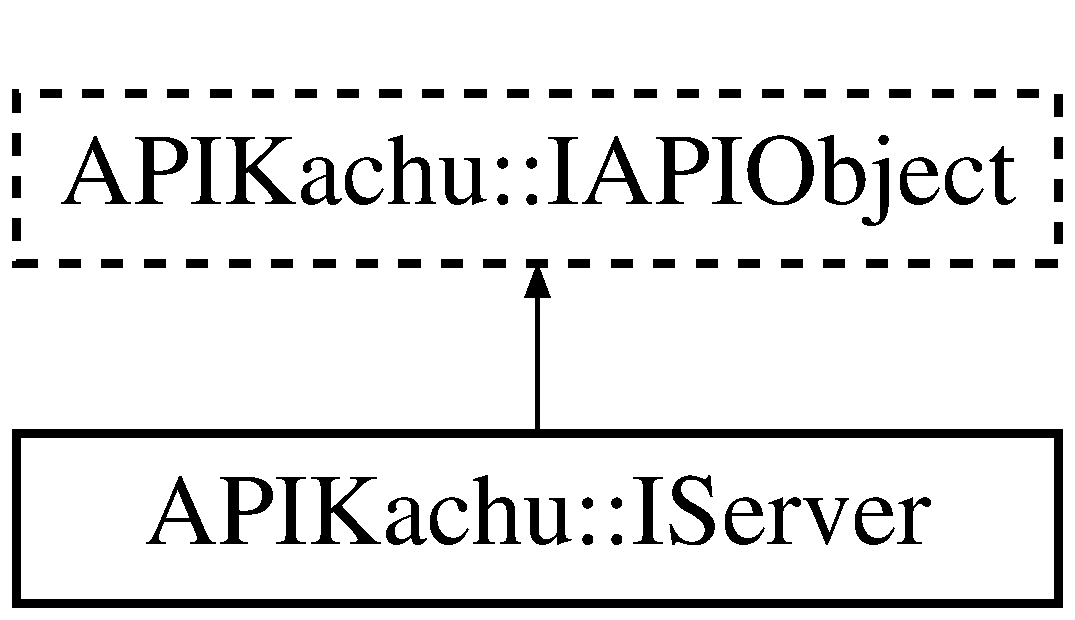
\includegraphics[height=2.000000cm]{class_a_p_i_kachu_1_1_i_server}
\end{center}
\end{figure}
\subsection*{Public Member Functions}
\begin{DoxyCompactItemize}
\item 
virtual const \hyperlink{class_a_p_i_kachu_1_1_i_config}{I\+Config} \& \hyperlink{class_a_p_i_kachu_1_1_i_server_a4a9d8cd045034108f204bf9617103af5}{get\+Config} () const  =0\hypertarget{class_a_p_i_kachu_1_1_i_server_a4a9d8cd045034108f204bf9617103af5}{}\label{class_a_p_i_kachu_1_1_i_server_a4a9d8cd045034108f204bf9617103af5}

\begin{DoxyCompactList}\small\item\em Getter for the configuration of the server. \end{DoxyCompactList}\item 
virtual \hyperlink{class_a_p_i_kachu_1_1_logger}{Logger} \& \hyperlink{class_a_p_i_kachu_1_1_i_server_af7a87851ad77ac1efdacb277ea2bec59}{get\+Logger} ()=0\hypertarget{class_a_p_i_kachu_1_1_i_server_af7a87851ad77ac1efdacb277ea2bec59}{}\label{class_a_p_i_kachu_1_1_i_server_af7a87851ad77ac1efdacb277ea2bec59}

\begin{DoxyCompactList}\small\item\em Getter for the logger of the server. \end{DoxyCompactList}\end{DoxyCompactItemize}


\subsection{Detailed Description}
Base interface for the server. 

Implements the basic methods used by the modules 

The documentation for this class was generated from the following file\+:\begin{DoxyCompactItemize}
\item 
Documents/bite/\+A\+P\+I-\/\+K\+A\+C\+H\+U/\+A\+P\+I/I\+Server.\+h\end{DoxyCompactItemize}

\hypertarget{class_a_p_i_kachu_1_1_logger}{}\section{A\+P\+I\+Kachu\+:\+:Logger Class Reference}
\label{class_a_p_i_kachu_1_1_logger}\index{A\+P\+I\+Kachu\+::\+Logger@{A\+P\+I\+Kachu\+::\+Logger}}


Base class for message displaying.  




{\ttfamily \#include $<$Logger.\+h$>$}

Inheritance diagram for A\+P\+I\+Kachu\+:\+:Logger\+:\begin{figure}[H]
\begin{center}
\leavevmode
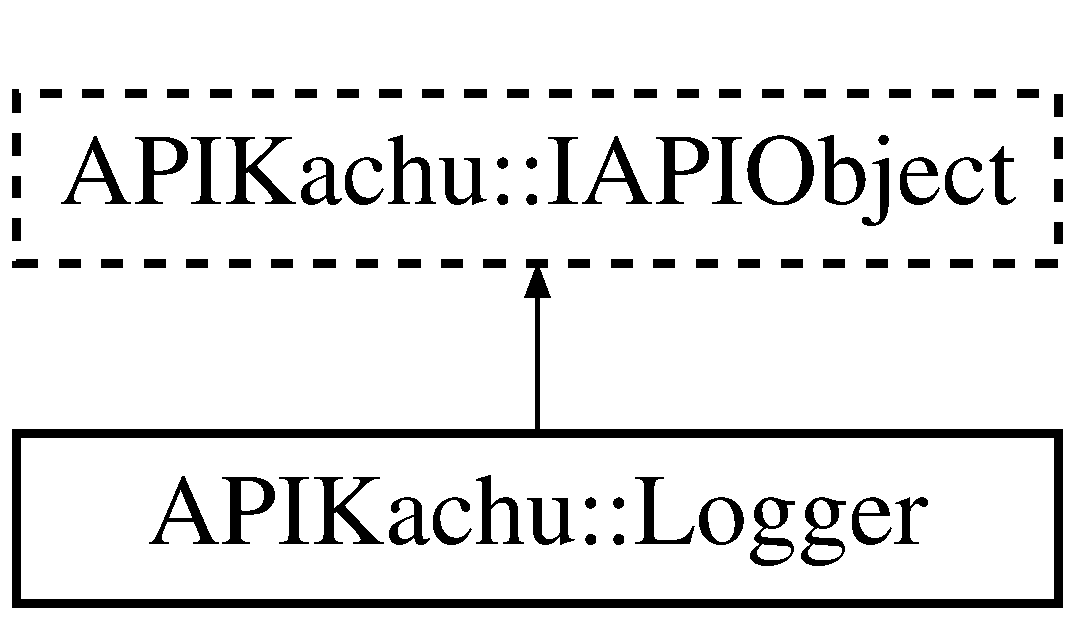
\includegraphics[height=2.000000cm]{class_a_p_i_kachu_1_1_logger}
\end{center}
\end{figure}
\subsection*{Public Types}
\begin{DoxyCompactItemize}
\item 
enum \hyperlink{class_a_p_i_kachu_1_1_logger_af1782b2d51f63b086775b671b3c8de52}{Log\+Type} \+: uint8 \{ \\*
{\bfseries L\+O\+G\+\_\+\+T\+Y\+P\+E\+\_\+\+N\+O\+NE} = 0x00, 
{\bfseries L\+O\+G\+\_\+\+T\+Y\+P\+E\+\_\+\+B\+A\+S\+IC} = 0x01, 
{\bfseries L\+O\+G\+\_\+\+T\+Y\+P\+E\+\_\+\+E\+R\+R\+OR} = 0x02, 
{\bfseries L\+O\+G\+\_\+\+T\+Y\+P\+E\+\_\+\+D\+E\+B\+UG} = 0x04, 
\\*
{\bfseries L\+O\+G\+\_\+\+T\+Y\+P\+E\+\_\+\+D\+E\+T\+A\+IL} = 0x08, 
{\bfseries L\+O\+G\+\_\+\+T\+Y\+P\+E\+\_\+\+A\+LL} = 0x\+FF
 \}\begin{DoxyCompactList}\small\item\em Type of a message to be logged. \end{DoxyCompactList}
\end{DoxyCompactItemize}
\subsection*{Public Member Functions}
\begin{DoxyCompactItemize}
\item 
\hyperlink{class_a_p_i_kachu_1_1_logger_a0f36a216974696dc4b5e55bfe77a1bfa}{Logger} (uint8 log\+Type)
\begin{DoxyCompactList}\small\item\em Constructor for the logger. \end{DoxyCompactList}\item 
virtual \hyperlink{class_a_p_i_kachu_1_1_logger_a8654a8cafaae01e3cdb8d8ba2bd9621a}{$\sim$\+Logger} ()=default\hypertarget{class_a_p_i_kachu_1_1_logger_a8654a8cafaae01e3cdb8d8ba2bd9621a}{}\label{class_a_p_i_kachu_1_1_logger_a8654a8cafaae01e3cdb8d8ba2bd9621a}

\begin{DoxyCompactList}\small\item\em Destructor for the logger. \end{DoxyCompactList}\item 
virtual void \hyperlink{class_a_p_i_kachu_1_1_logger_a71f7b72c8f52540468afd1eb0a9079cf}{set\+Log\+Type} (uint8 new\+Log\+Type)
\begin{DoxyCompactList}\small\item\em Setter for the log type. \end{DoxyCompactList}\item 
void \hyperlink{class_a_p_i_kachu_1_1_logger_a70dc2e7e6240a77054d33ca22b0ef1f9}{set\+File} (F\+I\+LE $\ast$file)
\begin{DoxyCompactList}\small\item\em Setter for the log file. \end{DoxyCompactList}\item 
{\footnotesize template$<$typename... Args$>$ }\\void \hyperlink{class_a_p_i_kachu_1_1_logger_ad74e704ae848ac5113e9a9e28337d455}{out\+Basic} (const char $\ast$format, const Args \&...args)
\begin{DoxyCompactList}\small\item\em Outputs a basic message. \end{DoxyCompactList}\item 
{\footnotesize template$<$typename... Args$>$ }\\void \hyperlink{class_a_p_i_kachu_1_1_logger_a6cbf04b8db00bcb707981722d67e1a8e}{out\+Error} (const char $\ast$format, const Args \&...args)
\begin{DoxyCompactList}\small\item\em Outputs an error message. \end{DoxyCompactList}\item 
{\footnotesize template$<$typename... Args$>$ }\\void \hyperlink{class_a_p_i_kachu_1_1_logger_a42e6ed2289a67d7c9b04558940e385e3}{out\+Debug} (const char $\ast$format, const Args \&...args)
\begin{DoxyCompactList}\small\item\em Outputs a debug message. \end{DoxyCompactList}\item 
{\footnotesize template$<$typename... Args$>$ }\\void \hyperlink{class_a_p_i_kachu_1_1_logger_ac310be8ea14351cba3c21b4ba770531a}{out\+Detail} (const char $\ast$format, const Args \&...args)
\begin{DoxyCompactList}\small\item\em Outputs a detail message. \end{DoxyCompactList}\item 
virtual uint8 \hyperlink{class_a_p_i_kachu_1_1_logger_a2ad6555c3e1c745da1aa824a9c59ae0c}{get\+Log\+Type} () const \hypertarget{class_a_p_i_kachu_1_1_logger_a2ad6555c3e1c745da1aa824a9c59ae0c}{}\label{class_a_p_i_kachu_1_1_logger_a2ad6555c3e1c745da1aa824a9c59ae0c}

\begin{DoxyCompactList}\small\item\em Getter for the log type. \end{DoxyCompactList}\end{DoxyCompactItemize}


\subsection{Detailed Description}
Base class for message displaying. 

\hyperlink{class_a_p_i_kachu_1_1_logger}{Logger} for outputting messages to the console or a file 

\subsection{Member Enumeration Documentation}
\index{A\+P\+I\+Kachu\+::\+Logger@{A\+P\+I\+Kachu\+::\+Logger}!Log\+Type@{Log\+Type}}
\index{Log\+Type@{Log\+Type}!A\+P\+I\+Kachu\+::\+Logger@{A\+P\+I\+Kachu\+::\+Logger}}
\subsubsection[{\texorpdfstring{Log\+Type}{LogType}}]{\setlength{\rightskip}{0pt plus 5cm}enum {\bf A\+P\+I\+Kachu\+::\+Logger\+::\+Log\+Type} \+: uint8}\hypertarget{class_a_p_i_kachu_1_1_logger_af1782b2d51f63b086775b671b3c8de52}{}\label{class_a_p_i_kachu_1_1_logger_af1782b2d51f63b086775b671b3c8de52}


Type of a message to be logged. 

Specifies different types of messages ; used as a bitmask in the configuration (see documentation for configuration) 

\subsection{Constructor \& Destructor Documentation}
\index{A\+P\+I\+Kachu\+::\+Logger@{A\+P\+I\+Kachu\+::\+Logger}!Logger@{Logger}}
\index{Logger@{Logger}!A\+P\+I\+Kachu\+::\+Logger@{A\+P\+I\+Kachu\+::\+Logger}}
\subsubsection[{\texorpdfstring{Logger(uint8 log\+Type)}{Logger(uint8 logType)}}]{\setlength{\rightskip}{0pt plus 5cm}A\+P\+I\+Kachu\+::\+Logger\+::\+Logger (
\begin{DoxyParamCaption}
\item[{uint8}]{log\+Type}
\end{DoxyParamCaption}
)\hspace{0.3cm}{\ttfamily [inline]}}\hypertarget{class_a_p_i_kachu_1_1_logger_a0f36a216974696dc4b5e55bfe77a1bfa}{}\label{class_a_p_i_kachu_1_1_logger_a0f36a216974696dc4b5e55bfe77a1bfa}


Constructor for the logger. 

Constructs the logger and assigns a type for filtering incoming messages 
\begin{DoxyParams}{Parameters}
{\em uint8} & logtype -\/ bitmask specifying message types to display \\
\hline
\end{DoxyParams}


\subsection{Member Function Documentation}
\index{A\+P\+I\+Kachu\+::\+Logger@{A\+P\+I\+Kachu\+::\+Logger}!out\+Basic@{out\+Basic}}
\index{out\+Basic@{out\+Basic}!A\+P\+I\+Kachu\+::\+Logger@{A\+P\+I\+Kachu\+::\+Logger}}
\subsubsection[{\texorpdfstring{out\+Basic(const char $\ast$format, const Args \&...\+args)}{outBasic(const char *format, const Args &...args)}}]{\setlength{\rightskip}{0pt plus 5cm}template$<$typename... Args$>$ void A\+P\+I\+Kachu\+::\+Logger\+::out\+Basic (
\begin{DoxyParamCaption}
\item[{const char $\ast$}]{format, }
\item[{const Args \&...}]{args}
\end{DoxyParamCaption}
)\hspace{0.3cm}{\ttfamily [inline]}}\hypertarget{class_a_p_i_kachu_1_1_logger_ad74e704ae848ac5113e9a9e28337d455}{}\label{class_a_p_i_kachu_1_1_logger_ad74e704ae848ac5113e9a9e28337d455}


Outputs a basic message. 

Only outputs a message if the logger\textquotesingle{}s log type contains L\+O\+G\+\_\+\+T\+Y\+P\+E\+\_\+\+B\+A\+S\+IC 
\begin{DoxyParams}{Parameters}
{\em const} & char $\ast$ format -\/ printf-\/type format \\
\hline
{\em ...} & -\/ arguments for the format \\
\hline
\end{DoxyParams}
\index{A\+P\+I\+Kachu\+::\+Logger@{A\+P\+I\+Kachu\+::\+Logger}!out\+Debug@{out\+Debug}}
\index{out\+Debug@{out\+Debug}!A\+P\+I\+Kachu\+::\+Logger@{A\+P\+I\+Kachu\+::\+Logger}}
\subsubsection[{\texorpdfstring{out\+Debug(const char $\ast$format, const Args \&...\+args)}{outDebug(const char *format, const Args &...args)}}]{\setlength{\rightskip}{0pt plus 5cm}template$<$typename... Args$>$ void A\+P\+I\+Kachu\+::\+Logger\+::out\+Debug (
\begin{DoxyParamCaption}
\item[{const char $\ast$}]{format, }
\item[{const Args \&...}]{args}
\end{DoxyParamCaption}
)\hspace{0.3cm}{\ttfamily [inline]}}\hypertarget{class_a_p_i_kachu_1_1_logger_a42e6ed2289a67d7c9b04558940e385e3}{}\label{class_a_p_i_kachu_1_1_logger_a42e6ed2289a67d7c9b04558940e385e3}


Outputs a debug message. 

Only outputs a message if the logger\textquotesingle{}s log type contains L\+O\+G\+\_\+\+T\+Y\+P\+E\+\_\+\+D\+E\+B\+UG 
\begin{DoxyParams}{Parameters}
{\em const} & char $\ast$ format -\/ printf-\/type format \\
\hline
{\em ...} & -\/ arguments for the format \\
\hline
\end{DoxyParams}
\index{A\+P\+I\+Kachu\+::\+Logger@{A\+P\+I\+Kachu\+::\+Logger}!out\+Detail@{out\+Detail}}
\index{out\+Detail@{out\+Detail}!A\+P\+I\+Kachu\+::\+Logger@{A\+P\+I\+Kachu\+::\+Logger}}
\subsubsection[{\texorpdfstring{out\+Detail(const char $\ast$format, const Args \&...\+args)}{outDetail(const char *format, const Args &...args)}}]{\setlength{\rightskip}{0pt plus 5cm}template$<$typename... Args$>$ void A\+P\+I\+Kachu\+::\+Logger\+::out\+Detail (
\begin{DoxyParamCaption}
\item[{const char $\ast$}]{format, }
\item[{const Args \&...}]{args}
\end{DoxyParamCaption}
)\hspace{0.3cm}{\ttfamily [inline]}}\hypertarget{class_a_p_i_kachu_1_1_logger_ac310be8ea14351cba3c21b4ba770531a}{}\label{class_a_p_i_kachu_1_1_logger_ac310be8ea14351cba3c21b4ba770531a}


Outputs a detail message. 

Only outputs a message if the logger\textquotesingle{}s log type contains L\+O\+G\+\_\+\+T\+Y\+P\+E\+\_\+\+D\+E\+T\+A\+IL 
\begin{DoxyParams}{Parameters}
{\em const} & char $\ast$ format -\/ printf-\/type format \\
\hline
{\em ...} & -\/ arguments for the format \\
\hline
\end{DoxyParams}
\index{A\+P\+I\+Kachu\+::\+Logger@{A\+P\+I\+Kachu\+::\+Logger}!out\+Error@{out\+Error}}
\index{out\+Error@{out\+Error}!A\+P\+I\+Kachu\+::\+Logger@{A\+P\+I\+Kachu\+::\+Logger}}
\subsubsection[{\texorpdfstring{out\+Error(const char $\ast$format, const Args \&...\+args)}{outError(const char *format, const Args &...args)}}]{\setlength{\rightskip}{0pt plus 5cm}template$<$typename... Args$>$ void A\+P\+I\+Kachu\+::\+Logger\+::out\+Error (
\begin{DoxyParamCaption}
\item[{const char $\ast$}]{format, }
\item[{const Args \&...}]{args}
\end{DoxyParamCaption}
)\hspace{0.3cm}{\ttfamily [inline]}}\hypertarget{class_a_p_i_kachu_1_1_logger_a6cbf04b8db00bcb707981722d67e1a8e}{}\label{class_a_p_i_kachu_1_1_logger_a6cbf04b8db00bcb707981722d67e1a8e}


Outputs an error message. 

Only outputs a message if the logger\textquotesingle{}s log type contains L\+O\+G\+\_\+\+T\+Y\+P\+E\+\_\+\+E\+R\+R\+OR 
\begin{DoxyParams}{Parameters}
{\em const} & char $\ast$ format -\/ printf-\/type format \\
\hline
{\em ...} & -\/ arguments for the format \\
\hline
\end{DoxyParams}
\index{A\+P\+I\+Kachu\+::\+Logger@{A\+P\+I\+Kachu\+::\+Logger}!set\+File@{set\+File}}
\index{set\+File@{set\+File}!A\+P\+I\+Kachu\+::\+Logger@{A\+P\+I\+Kachu\+::\+Logger}}
\subsubsection[{\texorpdfstring{set\+File(\+F\+I\+L\+E $\ast$file)}{setFile(FILE *file)}}]{\setlength{\rightskip}{0pt plus 5cm}void A\+P\+I\+Kachu\+::\+Logger\+::set\+File (
\begin{DoxyParamCaption}
\item[{F\+I\+LE $\ast$}]{file}
\end{DoxyParamCaption}
)\hspace{0.3cm}{\ttfamily [inline]}}\hypertarget{class_a_p_i_kachu_1_1_logger_a70dc2e7e6240a77054d33ca22b0ef1f9}{}\label{class_a_p_i_kachu_1_1_logger_a70dc2e7e6240a77054d33ca22b0ef1f9}


Setter for the log file. 


\begin{DoxyParams}{Parameters}
{\em F\+I\+LE} & $\ast$file -\/ log file ; null redirect to stdout or stderr for errors \\
\hline
\end{DoxyParams}
\index{A\+P\+I\+Kachu\+::\+Logger@{A\+P\+I\+Kachu\+::\+Logger}!set\+Log\+Type@{set\+Log\+Type}}
\index{set\+Log\+Type@{set\+Log\+Type}!A\+P\+I\+Kachu\+::\+Logger@{A\+P\+I\+Kachu\+::\+Logger}}
\subsubsection[{\texorpdfstring{set\+Log\+Type(uint8 new\+Log\+Type)}{setLogType(uint8 newLogType)}}]{\setlength{\rightskip}{0pt plus 5cm}void A\+P\+I\+Kachu\+::\+Logger\+::set\+Log\+Type (
\begin{DoxyParamCaption}
\item[{uint8}]{new\+Log\+Type}
\end{DoxyParamCaption}
)\hspace{0.3cm}{\ttfamily [inline]}, {\ttfamily [virtual]}}\hypertarget{class_a_p_i_kachu_1_1_logger_a71f7b72c8f52540468afd1eb0a9079cf}{}\label{class_a_p_i_kachu_1_1_logger_a71f7b72c8f52540468afd1eb0a9079cf}


Setter for the log type. 


\begin{DoxyParams}{Parameters}
{\em unit8} & new\+Log\+Type -\/ bitmask specifying message types to display \\
\hline
\end{DoxyParams}


The documentation for this class was generated from the following files\+:\begin{DoxyCompactItemize}
\item 
C\+:/\+Users/\+Mathieu/\+Documents/\+Git\+Hub/\+A\+P\+I-\/\+M\+E\+A\+L/\+A\+P\+I/Logger.\+h\item 
C\+:/\+Users/\+Mathieu/\+Documents/\+Git\+Hub/\+A\+P\+I-\/\+M\+E\+A\+L/\+A\+P\+I/Logger.\+cpp\end{DoxyCompactItemize}

%--- End generated contents ---

% Index
\backmatter
\newpage
\phantomsection
\clearemptydoublepage
\addcontentsline{toc}{chapter}{Index}
\printindex

\end{document}
